\documentclass[../main/main.tex]{subfiles}
\begin{document}

%%%%%%%%%%%%%%%%%%%%%%%
%%%%%%%% LECTURE 11 %%%%%%%%
%%%%%%%%%%%%%%%%%%%%%%%

\chapter{Quantum solitons}

\section{Introduction to topological objects}

The first appearance of a classical \emph{soliton} was in a report by J. Scott Russel in 1842, he was in a boat in a channel and noticed ``a solitary elevation, a rounded, smooth and well-defined heap of water which continued in course along the channel apparently without change of form (i.e. without dispersion/dissipation) or diminution of speed (i.e. constant velocity). 

The term ``soliton'' (which comes from ``solitary wave'') was much later introduced to characterize solutions of wave equations that do not dispense and preserve their form during the propagation. Hence in a sense a classical solution behaves as a particle in spite of being a wave. 

The staticity of these ``wave'' solitons is due to some conservation law. If this conservation law is of topological origin (i.e. the conserved quantity is not related to the (first) Noether theorem and the conservation holds without using all the equations of motion\footnote{For instance, the conservation of the EM current $J_\nu=\partial^\mu F_{\mu\nu}$ does not follow from the equation of motion $\der{p^\mu}{t}=F^{\mu\nu}u_\nu$, but is just a consequence of the antisymmetry of $F_{\mu\nu}$: $\partial^\nu J_\nu=\partial^\mu\partial^\nu F_{\mu\nu}=\partial^{\{\mu}\partial^{\nu\}}F_{[\mu\nu]}=0$.}) these solitons are called \emph{topological}. 

The original concept of topologically protected ``wave'' solitons has been later extended, in particular by high-energy physicists, and today we define a classical topological soliton as a topologically stable, finite energy solution of the Hamiltonian equations of motion of a classical field theory. 

Since already classically solutions behaves as particles, one can naturally expect, correctly, that their quantized version provides a quantum particle, but as we will see later it is a peculiar one. 

\section{Spontaneously broken symmetry}\label{sec:SSB}

\cite[Chapter C.1]{Strocchi_1985}, \cite{Strocchi:2012}, \cite[Chapter 1]{Shifman:2012}\\

Before entering in the discussion of solitons, a brief formal discussion of the spontaneously broken symmetry (SSB) phenomenon is required. 

We already know that the \emph{observables} of a system are the quantities of the physical system that we can measure and the algebra that they generate is called the \emph{observable algebra} $\obsalg$. The \emph{states} contain the information on the system, if the information is maximal they are called \emph{pure}, if it is not maximal are said \emph{mixed}. 

By definition pure states can be obtained one from the other by operations physically performed on the system (including limiting procedure, such as the infinite volume limit or the thermodynamic limit, but excluding transformations which require to cross would-be states of infinite ). Both in the classical and quantum settings the mixed states can be viewed as complex combinations of pure states and a state is pure if it cannot be written as convex combination of the pure states. 
For equilibrium states at finite temperature by analogy we introduce the concept of \emph{pure phase}: an equilibrium state is a pure phase if it cannot be written as a convex combination of other equilibrium states.

\skipline

For instance consider the Ising model: take a finite lattice of volume $V$, where to each cell $i$ is associated a classical spin $\sigma_i$ with possible values $\pm1$. Suppose that we imposed vanishing boundary conditions, i.e. outside the volume we do not have any spin (the system is confined), and try to take the infinite volume limit. For spatial dimension $d=2$ and temperature $T<T_c$ where $T_c$ is the \emph{critical temperature} the system has two possible ground states: for the first one $\langle\sigma_i\rangle>0$ for all the cells, for the second one $\langle\sigma_i\rangle<0$. Obviously, the equilibrium state for the system in such condition is described by $\langle\sigma_i\rangle =0$ for all the possible cells, and it is not a pure phase as it can be described as a convex combination of the two ground states, which in turn are (unstable) equilibrium states. 

\skipline

We can now distinguish different kinds of symmetries. An \emph{algebraic symmetry} is an invertible algebra homomorphism $\obsalg\to\obsalg$ (i.e. a map preserving the algebraic relations, e.g.  equations of motion are preserved in form and also (in quantum setting) the commutation relations between observables). A \emph{physical symmetry} is an algebraic symmetry together with an invertible map $\purstate\to\purstate$, where $\purstate$ is the space of pure states, which preserves the expectation values:
\begin{eq}
	\begin{aligned} 
		\alpha:\obsalg&\longrightarrow\obsalg\\
		A&\longmapsto A'
	\end{aligned}
	\qquad\text{and}\qquad
	\begin{aligned}
		\tilde \alpha:\purstate&\longrightarrow\purstate\\
		\Sigma&\longmapsto\Sigma'
	\end{aligned}
\end{eq}
such that
\begin{eq}
	\langle A\rangle_\Sigma=\langle A'\rangle_{\Sigma'}
\end{eq}
A \emph{dynamical symmetry} is either an algebraic or a physical symmetry leaving the Hamiltonian invariant
\begin{eq}
	H\longmapsto H'=H
\end{eq}

A dynamical symmetry is said \emph{spontaneously broken} if it cannot be realized as a physical symmetry, i.e. is an algebraic symmetry leaving $H$ invariant but it does no exists a map in the space of pure states of the system preserving the expectation values. 

\skipline

Naively it seems impossible to define a spontaneously broken symmetry, as for each map $\alpha:\obsalg\to\obsalg$ always exists a map $\tilde\alpha:\purstate\to\purstate$ defined by
\begin{eq}
	\langle \alpha^{-1}(A)\rangle_\Sigma=\langle A\rangle_{\tilde\alpha(\Sigma)}
\end{eq}
which clearly implies
\begin{eq}
	\langle A\rangle_\Sigma=\langle\alpha(A)\rangle_{\tilde\alpha(\Sigma)}=\langle A'\rangle_{\Sigma'}
\end{eq}
What goes wrong is that such map $\tilde\alpha:\Sigma\mapsto\Sigma'$ in principle may send the space $\purstate$ not in itself, i.e. in principle $\tilde\alpha(\Sigma)\not\in\purstate$, but in another space of states not realizable by means of physical operations on the system starting from the initial states in $\purstate$.

\skipline

Take for instance the Heisenberg model of a ferromagnet in three dimension, where the spin is classically described by a unit vector in a lattice. Let's then consider the thermodynamic limit. It is well known that such system has a critical temperature $T_c$, such that for $T<T_c$ the ground states have an expectation value $\langle\vec s_i\rangle\neq0$. For $T=0$ all the spin are aligned in the same direction. The Hamiltonian for this system is 
\begin{eq}
	H=J\sum_{\langle i,j\rangle}(\vec s_i-\vec s_j)^2
\end{eq} 
which is clearly invariant under rotations. Consider two ground states at $T=0$ which differs for the orientation of the spins, and let's see if these can be related by some allowed transformation or not, if not we would have a spontaneous symmetry breaking. We are allowed to do only physical allowed (in particular, local) transformations, at least by some limiting procedure. Nevertheless we already took the thermodynamic limit, therefore we are not allowed to move all the spins (including those at infinity) at the same time with a single transformation. We are forced to use some limiting procedure, for instance we can consider neighbourhoods of circles of radius $R$ and smoothly rotate the spins in these regions, while we increase $R$ from 0 to $\infty$. But as $R$ approaches $\infty$ there are infinitely many spins rotated simultaneously, hence due to the non trivial interacting energy between spins, one can expect that such procedure requires an infinite amount of energy. If the explicit computation of the energy actually give us an infinite energy cost, then spontaneous symmetry breaking occured. 

Notice that in general one cannot guess whether we have SSB or not, a computation of the energy (or some other relevant physical quantity) is needed. 

\skipline

Unfortunately sometimes one refers to SSB in the case in which the Hamiltonian is invariant under a symmetry $\alpha$, but each of its pure equilibrium states are not invariant under $\tilde\alpha$, hence restricting the non-invariance to equilibrium states. 

For field theories are basically equivalent from the practical point of view but for systems with finite degrees of freedom they are not. For instance consider a horizontal place where gravitational force applies in the vertical direction, and put a point particle at rest a point, then certainly this describes an equilibrium state. The Hamiltonian is invariant under horizontal space translations, nevertheless the equilibrium state is not, hence according to the latter definition the symmetry is spontaneously broken. On the other side, certainly this is not a SSB according to the first definition, because we can easily move to another equilibrium state by some physically allowed translation, since all the intermediate states are pure states of the system. 

\chapter{Kinks}

\cite[Chapter 2]{Shifman:2012}, \cite{Gousheh_2012}, \cite[Chapters 2,5,8]{Rajaraman:1982}\\

The fist (topological) soliton that we consider is the \emph{kink} in $\phi^4_2$, i.e. the relativistic $\phi^4$ theory in 1+1 dimensions in the spontaneously broken phase. 

\section{Classical treatment}

The classical Hamiltonian we consider is on the real line $\R$, labelled by $x$, and if the system is described by a real scalar field $\phi(x,t)$ with conjugated momentum $\pi(x,t)$ (the dependence on time of the fields is understood) it reads
\begin{eq}\label{eq:ham-kink}
	H=\int\de x\,\ham\big(\pi,\phi\big)=\int\de x\,\left[\half\pi^2+\half\left(\der{\phi} x\right)^2+\frac{g^2}4\big(\phi^2-v^2\big)^2\right]
\end{eq}
with $v,g\in\R$. This potential is the field analogue of the double well with potential $\frac{g^2}4(x^2-v^2)^2$.
The equations of motion in Hamiltonian formalism are
\begin{eq}
	\dphi&=\fder{H}{\pi}=\pder{\ham}{\pi}=\pi\\
	\dpi&=\fder{H}{\phi}=\pder{\ham}{\phi}=-\dpder{}{x}\phi+g^2\big(\phi^2-v^2\big)\phi
\end{eq}
where for the second equation we used an appropriate integration by parts in $H$. 
Equilibrium states are given by the equilibrium condition $\dphi=\dpi=0$, which implies (for each $x\in\R$)
\begin{eq}
	\pi=0
	\tand
	\dpder{}{x}\phi=g^2\big(\phi^2-v^2\big)\phi
\end{eq}
Clearly, from the structure of the Hamiltonian, finite energy solutions must satisfy 
\begin{eq}\label{eq:kink-boundary-conditi}
	\pi\to0
	\tand
	\phi\to\pm v
	\tfor
	x\to\pm\infty
\end{eq}
as otherwise $H$ is divergent. Indeed all the terms inside $H$ are strictly positive, hence both the term depending on $\pi$ and the term depending on $\phi$ should vanish identically at infinite. The absolute minima of $H$ are given by the two configurations
\begin{eq}
	\phi_+^0=+v \tcomma \pi^0=0
	\tand
	\phi_-^0=-v \tcomma \pi^0=0
\end{eq}
In such cases $H$ vanishes, hence both these solutions are called \emph{vacuum}. The expectation values of the field at the minima are
\begin{eq}
	\langle\phi\rangle_{\phi_\pm^0,\pi^0}=\pm v
\end{eq}

\skipline

The Hamiltonian is invariant under the symmetry $\alpha$
\begin{eq}\label{eq:symm_kink}
	\phi\mapsto-\phi
	\tcomma
	\pi\mapsto-\pi
\end{eq}
We see that in order to satisfy
\begin{eq}
	\langle\phi\rangle_\Sigma=\langle\alpha(\phi)\rangle_{\tilde\alpha(\Sigma)}
\end{eq}
for $\Sigma=(\phi^0_\pm,\pi^0)$ we should have 
\begin{eq}
	\pm v=\langle-\phi\rangle_{\tilde\alpha(\phi^0_\pm, \pi^0)}
\end{eq}
which is satisfied for $\tilde\alpha(\phi^0_\pm,\pi^0)=(\phi^0_\mp,\pi^0)$.
However it is impossible to reach continuously $\phi_-^0$ from $\phi_+^0$ and vice versa, since the set of boundary conditions at infinity, $\{+v,-v\}$, is not connected and to reach one minimum from the other with (the limit of) a local transformation we need to cross infinite energy states. Therefore symmetry eq.~\eqref{eq:symm_kink} is spontaneously broken, and the two minima that we found lives in disjoint space of states related by a parity transformation.

\subsubsection{First-order equation}

However there are two local minima in the space of finite-energy solutions: we can find them with the following trick. For $\pi=\dphi=0$ the equation of motion reduces to
\begin{eq}\label{eq:eom-kink}
	\der{^2}{x^2}\phi=\frac{g^2}4(\phi^2-v^2)\phi
\end{eq}
where now $\phi$ depends only on $x$. If we think about $x$ as a time coordinate and $\phi$ as the position $q$  of a particle, then eq.~\eqref{eq:eom-kink} become a Newton equation with potential $V(q)=\frac{g^2}4(q^2-v^2)^2$. Due to energy conservation we get
\begin{eq}
	\half\dot q^2-\frac{g^2}4(q^2-v^2)^2=\tconst=0
\end{eq}
where the vanishing of the energy is due to the boundary condition eq.~\eqref{eq:kink-boundary-conditi}. Hence we can solve the previous differential equation:
\begin{eq}
	\der qt=\pm\frac g{\sqrt2}(q^2-v^2)
\end{eq}
i.e.
\begin{eq}
	\der\phi x=\pm\frac g{\sqrt2}(\phi^2-v^2)
\end{eq}
These are standard first order equations trivially solved by 
\begin{eq}
	\int\de x=\mp\frac{\sqrt2}{g}\int\frac{\de\phi}{\phi^2-v^2}
\end{eq}
which have solutions
\begin{eq}
	x=\pm\frac{\sqrt2}{gv}\arctanh\left(\frac\phi v\right)+x_0
\end{eq}
i.e.
\begin{eq}
	\phi_\pm^S(x)=\pm v\tanh\left(\frac{gv}{\sqrt2}(x-x_0)\right)
\end{eq}
where we denoted the two solutions by $S$, which means ``soliton''. In fig.~\ref{fig:kink-solution} one can find a plot of the function $\phi_+^S(x)$. The value $x_0$ is called \emph{collective coordinate} or the \emph{modulus} of the soliton, called (classical) \emph{kink} ($\phi_+^S(x)$) or (classical) \emph{anti-kink} ($\phi_-^S(x)$).

\begin{figure}[h]
\centering
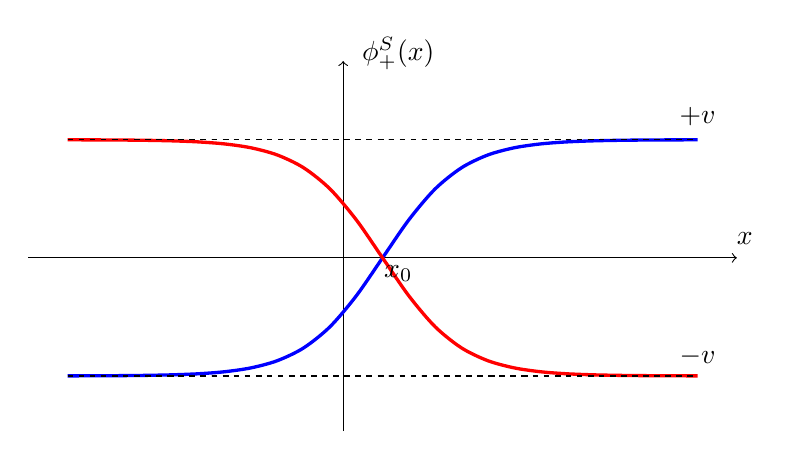
\begin{tikzpicture}
  \draw[->] (-4, 0) -- (5, 0) node[at={(5.1,0.25)}] {$x$};
  \draw[->] (0, -2.2) -- (0, 2.5) node[at={(0.7,2.6)}] {$\phi_+^S(x)$};
  \draw[scale=0.5, domain=-7:9, smooth, variable=\x, blue, very thick] plot ({\x}, {3*tanh(0.5*(\x-1))});
    \draw[scale=0.5, domain=-7:9, smooth, variable=\x, red, very thick] plot ({\x}, {-3*tanh(0.5*(\x-1))});
  \draw[scale=0.5, domain=-7:9, smooth, variable=\x, dash pattern=on 2pt off 2pt] plot ({\x}, {3});
  \draw[scale=0.5, domain=-7:9, smooth, variable=\x, dash pattern=on 2pt off 2pt] plot ({\x}, {-3});
  \draw (4.5,1.8) node {$+v$};
  \draw (4.5,-1.25) node {$-v$};
  \draw (0.7,-0.2) node {$x_0$};
\end{tikzpicture}
\caption{Shape of the solutions $\phi_+^S(x)$ (blue) and $\phi_-^S(x)$ (red).} %parameters: x_0=1, v=3, g=1/3sqrt2 
\label{fig:kink-solution}
\end{figure}

We see that $\phi_+^S$, $\phi_-^S$, $\phi_+^0$ and $\phi_-^0$ cannot be deformed one into other by operations physically implementable, since the boundary conditions at $\infty$ are disjoint. This statement can be translated for the solitons in the conservation of a charge
\begin{eq}\label{eq:cons-charge-kink}
	Q=\int\de x\der{}{x}\phi=\phi(+\infty)-\phi(-\infty)
\end{eq}
which is topological (only the behaviour at infinity is relevant). The corresponding conserved current is 
\begin{eq}
	J_\mu(x)=\lctens_{\mu\nu}\partial^\nu\phi
\end{eq}
with $\mu,\nu=0,1$ where $\mu=0$ is the time $t$ component and $\mu=1$ is the spatial $x$ component, moreover $\lctens$ is the Levi-Civita tensor. We can easily see that $J_0$ actually coincides with the conserved density associated to \eqref{eq:cons-charge-kink}:
\begin{eq}
	\int\de x\, J_0=\int\de x \,\lctens_{0\nu}\partial^\nu\phi=
	\int\de x \,\partial^1\phi=\int\de x\,\pder{}x\phi=Q
\end{eq}
while $J_1$ is the unique component of the vector current. The current $J_\mu$ is automatically conserved without using the equations of motion, since the conservation directly follows from the contraction of a symmetric tensor with an antisymmetric one
\begin{eq}
	\partial^\mu J_\mu=\lctens_{\mu\nu}\partial^\mu\partial^\nu\phi=\lctens_{[\mu\nu]}\partial^{\{\mu}\partial^{\nu\}}\phi=0
\end{eq}

%%%%%%%%%%%%%%%%%%%%%%%
%%%%%%%% LECTURE 12 %%%%%%%%
%%%%%%%%%%%%%%%%%%%%%%%

\subsubsection{The Bogomol'nyi bound}

There is a more instructive way to prove that $\phi_\pm^S$ are the local minima at $(\mp v,\pm v)$ boundary conditions. Let's write the potential $V(\phi)$ in terms of a function $\suppot(\phi)$ called \emph{superpotential} (since it is largely used in supersymmetric theories) by
\begin{eq}
	V(\phi)=\half\left(\der\suppot\phi\right)^2
\end{eq}
Since $V(\phi)=\frac{g^2}4(\phi^2-v^2)^2$ this implies that
\begin{eq}
	\der\suppot\phi=\frac g{\sqrt2}(\phi^2-v^2)
	\tand
	\suppot=\frac g{\sqrt2}\left(\frac13\phi^3-v^2\phi\right)
\end{eq}
The Hamiltonian can be rewritten for $\pi=0$ as
\begin{eq}\label{eq:Ham-kink-suppot}
	H=\int\de x\,\left[\half\left(\der\phi x\pm\der\suppot\phi\right)^2\mp\der\phi x\der\suppot\phi\right]
	\quad\text{for boundary conditions }(\mp v,\pm v)
\end{eq}
Now notice that the last term gives
\begin{eq}
	&\int\de x\,\der\suppot\phi\der\phi x=\suppot(\phi(+\infty))-\suppot(\phi(-\infty)
	=\pm\Delta\suppot\quad\text{for boundary conditions }(\mp v,\pm v)
\end{eq}
with
\begin{eq}
	\Delta\suppot=\suppot(v)-\suppot(-v)=-\frac4{3\sqrt2}gv^3<0
\end{eq}
hence we get that
\begin{eq}\label{eq:Bogom-bound}
	H\geq-\Delta\suppot>0
\end{eq}
for both the possible boundary conditions. This lower bound  is called \emph{Bogomol'nyi bound} (as we will see has several generalizations). This bound is saturated, hence the equality in eq.~\eqref{eq:Bogom-bound} holds, only if the term inside square brackets in eq.~\eqref{eq:Ham-kink-suppot} vanishes, i.e. if the following first order equation is satisfied
\begin{eq}\label{eq:Bogom-bound-cond}
	\der\phi x=\pm\der\suppot\phi
\end{eq}
which coincides exactly with eq.~\eqref{eq:eom-kink}. Hence the solutions $\phi_\pm^S$ are local minima for which the energy coincides with the Bogomol'nyi bound. 

\skipline

The energy density associated to $\phi_\pm^S(x_0)$, depending on the modulus $x_0$, is given by the Hamiltonian density evaluated for the field $\phi_\pm^S(x_0)$ (it obviously depends on the spatial coordinate $x$ and on the choice of $x_0$):
\begin{eq}\label{eq:kink-classic-energy-density}
	\cenergy^\tcl&=\half\left(\der{\phi_\pm^S}x\right)^2+\frac{g^2}4\left(\phi_\pm^{S\,2}-v^2\right)^2
	\overset{\eqref{eq:Bogom-bound-cond}}=2\cdot\half\left(\der{\phi_\pm^S}x\right)^2=\left(\der{\phi_\pm^S}x\right)^2
\end{eq}
In fig.~\ref{fig:kink-energy} one can see the shape of $\cenergy(x)$ associated to the field of fig.~\ref{fig:kink-solution}. It is clearly localized near $x_0$. Hence the soliton exhibits an energy density profile as a `` dump'' around $x_0$, thus behaving ``like a particle'' localized around $x_0$. The integral 
\begin{eq}\label{eq:mass-classical-kink}
	M_S^\tcl:=\int\de x\,\cenergy^\tcl(x)=-\Delta\suppot=\frac4{3\sqrt2}gv^3
\end{eq}
can be interpreted as the ``classical'' mass of the soliton, i.e. the energy of the soliton in its rest frame. 

\begin{figure}[h]
\centering
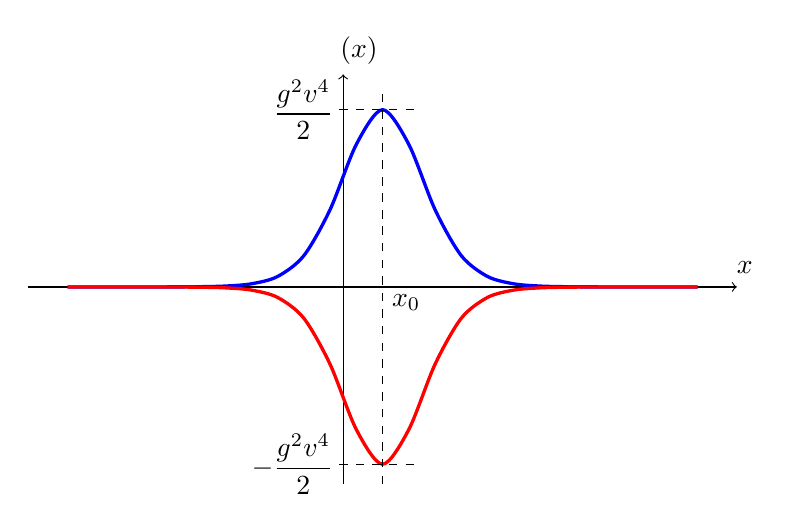
\begin{tikzpicture}
  \draw[->] (-4, 0) -- (5, 0) node[at={(5.1,0.25)}] {$x$};
  \draw[->] (0, -2.5) -- (0, 2.7) node[at={(0.2,3)}] {$\cenergy(x)$};
  \draw[scale=0.5, domain=-7:9, smooth, variable=\x, blue, very thick] plot ({\x}, {4.5*(cosh((\x-1)/2))^(-4)});
  \draw[scale=0.5, domain=-7:9, smooth, variable=\x, red, very thick] plot ({\x}, {-4.5*(cosh((\x-1)/2))^(-4)});
   \draw[scale=0.5, domain=-5:5, smooth, variable=\y, dash pattern=on 3pt off 3pt] plot ({1}, {\y});
   \draw[scale=0.5, domain=-0.1:2, smooth, variable=\x, dash pattern=on 3pt off 3pt] plot ({\x}, {4.5});
   \draw[scale=0.5, domain=-0.1:2, smooth, variable=\x, dash pattern=on 3pt off 3pt] plot ({\x}, {-4.5});
  \draw (0.8,-0.2) node {$x_0$};
  \draw (0,2.25) node [anchor=east]{$\displaystyle\frac{g^2v^4}2$};
  \draw (0,-2.25) node [anchor=east]{$\displaystyle-\frac{g^2v^4}2$};
\end{tikzpicture}
\caption{Shape of the energy density for the fields $\phi_+^S(x)$ (blue) and}{$\phi_-^S(x)$ (red) plotted in fig.~\ref{fig:kink-solution} (the $x$-axis has not been rescaled).} %parameters: x_0=1, v=3, g=1/3sqrt2 
\label{fig:kink-energy}
\end{figure}

Since (looking at the Hamiltonian) the theory is Lorentz invariant (on 1+1 dimension) one can ``change the reference frame'' and make the soliton move at a constant velocity $\textrm v$:
\begin{eq}
	\phi_\pm^S(x,x_0,\textrm v)=\pm v\tanh\left(\frac{gv}{\sqrt2}\,\frac{x-x_0-\textrm vt}{\sqrt{1-\textrm v^2}}\right)
\end{eq}
i.e. behaves like a particle with equation of motion $x=x_0+\textrm vt$.

\section{Semi-classical treatment}

Up to now we just described the soliton at classical level. Let us turn to the quantum world. We first give a standard semi-classical (heuristic) Hamiltonian treatment, then we make some comments on a rigorous approach in the spirit of the reconstruction theorem previously discussed. 

\subsubsection{Semi-classical description of fluctuations around the vacuum}

Let us start from the quantization of fluctuations around one vacuum. To quantize perturbatively fluctuations around $\phi_+^0=v$ we rewrite the quantum field as
\begin{eq}
	\ophi(x)=v+\ochi(x)
\end{eq}
Formally (in principle regularizations are needed) expanding in $\ochi$ in the Hamiltonian we get
\begin{eq}	
	H&=\int\de x\,\left[\frac12\opi^2+\frac12\left(\der\ochi x\right)^2+\frac{g^2}4\left(2v\ochi+\ochi^2\right)^2\right]\\
	&=\int\de x\,\left[\frac12\opi+\frac12\left(\der\ochi x\right)^2+\frac{2(gv)^2}2\ochi^2+\polyn(\ochi)\right]
\end{eq}
where $\polyn(\ochi)$ is a polynomial in $\ochi$ of order higher than 2. Integrating by part we get
\begin{eq}
	H_2=\int\de x\,\left[\frac12\opi+\frac12\ochi\left(-\der{^2}{x^2}+2(gv)^2\right)\ochi\right]
\end{eq}
($H_2$ denotes the quadratic part on $H$, describing the free field). One can then expand $\ochi$ in terms of the complete set of solutions of the differential equation
\begin{eq}
	\left(-\der{^2}{x^2}+2(gv)^2\right)\chi_k=\omega^2(k)\chi_k
\end{eq}
which we know are just the complex exponentials $e^{ikx}$ with eigenvalues
\begin{eq}
	\omega^2(k)=k^2+2(gv)^2
\end{eq}
and then one can write
\begin{eq}
	\ochi(x)=\sum_k\op a(k)\chi_k(x)
\end{eq}
From the quadratic terms we see that $\ochi$ is a massive field with (bare) mass $m=\sqrt2gv$, such that we recover the usual dispersion relation $\omega(k)=\sqrt{k^2+m^2}$, and polynomial interaction given by $\polyn(\ochi)$.

Perturbatively we impose the CCR on $\ochi$ and $\opi=\dot\ochi$
\begin{eq}
	[\ochi(x),\opi(y)]=[\ochi(x),\dot\ochi(y)]=i\hbar\,\delta(x-y)
\end{eq}
and in order to make sense to the previous discussion we insert a normal ordering in the Hamiltonian, so that the free $H_2$ Hamiltonian has zero vacuum energy (otherwise it would be divergent) and then proceed in the usual way. 

Clearly in perturbation theory the bare mass of $\ochi$ is renormalized by the polynomial interaction, and the relevant term, coming from $\nord{\ochi^4\!}$, is the counterterm corresponding to the following Feynman graph

\begin{eq}\label{eq:correct-mass-kink-vacuum}
	(-1)\cdot\quad\begin{tikzpicture}[baseline=($(a)+(-90:0.1)$)]	
		\coordinate (a) at (-1.6,0);
		\coordinate (b) at (0,0);
		\coordinate (c) at (1.6,0);	
		\draw (a) -- (c);
		\draw ($(b)+(90:0.6)$) circle(0.6);
		\draw ($(b)+(-90:0.4)$) node {$\displaystyle{g^2}/4$};
		\filldraw [black] (b) circle (2pt);
		\draw ($(a)+(90:0.3)$) node {$\chi$};
		\draw ($(c)+(90:0.3)$) node {$\chi$};
		\draw ($(b)+(90:1.5)$) node {$\chi$};
	\end{tikzpicture}
	\quad=\quad-4\cdot3\cdot\frac{g^2}4\int\frac{\de^2p}{(2\pi)^2}\frac\hbar{p^2+m^2}
	=-\frac{3g^2}{4\pi}\int_0^\infty\de p\der{}{p}\log(p^2+m^2)
\end{eq}
where $4\cdot 3$ is a combinatorial factor\footnote{Notice that the coupling $\frac {g^2}4$ already contains the factor $1/4!$ associated to the possible permutations of the legs of the vertex. This can be easily understood by comparing the interaction potential of the theory with the potential of $\lambda\phi^4$ theory. Since there is only one vertex in the graph no symmetry factor associated to the exchange of the vertices is needed. Hence we just have to take care of the $4\cdot3$ possible ways to connect the external fields to the vertex.}, and we set $\hbar=1$. Introducing a cutoff $\Lambda\gg m$ we get renormalized mass
\begin{eq}\label{eq:classical-mass-kink}
	m^2_R=m^2-\frac{3g^2}{2\pi}\log(\frac{\Lambda^2}{m^2})
\end{eq}
where we multiplied the correction coming from \eqref{eq:correct-mass-kink-vacuum} by 2 in order to take into account the factor 1/2 in the mass term of the Hamiltonian. The quantity $m^2_R$ is exactly the square of the mass that one detects if perform an experimental measure of the mass of the fluctuation $\chi$ around the vacuum. 

\subsubsection{Semi-classical description of fluctuations around soliton solution}

Let us now turn to the quantization around the soliton solution, consider for instance $\phi_+^S$. Since this is a local minima, we can still expand around such solution very similarly to what we done for the fluctuations around the vacuum. First notice that, expressed in terms of the bare mass $m=\sqrt2gv$, the classical mass of the kink eq.~\eqref{eq:mass-classical-kink} reads
\begin{eq}
	M^\tcl_S=\frac {m^3}{3g^2}\sim\frac1{g^2}
\end{eq}
hence it cannot be recovered by a perturbation theory around $g=0$, the perturbative expansion in $g^{-2}$ is not well defined for $g\approx0$. The behaviour $\sim g^{-2}$ of the energy or the action is typical to the soliton solutions. 

A naive approach to quantization would be to write
\begin{eq}
	\ophi(x,t)=\phi_+^S(x)+\ochi(x,t)
\end{eq}
Inserting in the Hamiltonian we get
\begin{eq}
	H &= \int\de x\bigg[\,\half{{\dot\phi^S_+}\hspace{0cm}}^2+\dot\phi^S_+\dot\ochi+\half\dot\ochi^2+\half\left(\der{{\phi_+^S}}x\right)^2+\der{{\phi_+^S}}x\der\ochi x+\half\left(\der\ochi x\right)^2+\\
	&\qquad+\frac{g^2}4\left[({\phi_+^S}^2-v^2)^2+(4{\phi_+^S}^3-4v^2{\phi_+^S})\ochi+(6{\phi_+^S}^2-2v^2)\ochi^2+4{\phi_+^S}\ochi^3+\ochi^4\right]\bigg]
\end{eq}
By integrating by parts with boundary conditions $\ochi(\pm\infty)=0$ (otherwise the field would have infinite energy) we get
\begin{eq}
	H&= \int\de x\bigg[\,\half{{\dot\phi^S_+}{}}^2+\dot\phi^S_+\dot\ochi+\half\dot\ochi^2+\half\left(\der{{\phi_+^S}}x\right)^2-\der{^2\phi_+^S}{x^2}\,\ochi-\half\ochi\,\der{^2\ochi}{x^2}+\\
	&\qquad+\frac{g^2}4\left[({\phi_+^S}^2-v^2)^2+(4{\phi_+^S}^3-4v^2{\phi_+^S})\ochi+(6{\phi_+^S}^2-2v^2)\ochi^2+4{\phi_+^S}\ochi^3+\ochi^4\right]\bigg]
\end{eq}
first notice that the terms linear in $\ochi$ vanish due to the equation of motion of $\phi_+^S$:
\begin{eq}
	\left(\der{^2\phi_+^S}{x^2}-{g^2}({\phi_+^S}^3-v^2\phi_+^S)\right)\ochi=0
\end{eq}
and combining with \eqref{eq:kink-classic-energy-density} we get
\begin{eq}\label{eq:full_ham_fluc}
	H&= M_S^\tcl+\int\de x\bigg[\,\half{{\dot\phi^S_+}\hspace{0cm}}^2+\dot\phi^S_+\dot\ochi+\half\dot\ochi^2-\half\ochi\,\der{^2\ochi}{x^2}+\frac{g^2}4\left[(6{\phi_+^S}^2-2v^2)\ochi^2+4{\phi_+^S}\ochi^3+\ochi^4\right]\bigg]\\
	&=M_S^\tcl+\int\de x\bigg[\,\half{{\dot\phi^S_+}\hspace{0cm}}^2+\dot\phi^S_+\dot\ochi+\half\dot\ochi^2+\half\ochi L_2\ochi+\frac{g^2}4\left(4{\phi_+^S}\ochi^3+\ochi^4\right)\bigg]
\end{eq}	
with
\begin{eq}
	L_2=\frac{g^2}2(6{\phi_+^S}^2-2v^2)-\der{^2}{x^2}=\frac{m^2}{2}\left(3\tanh^2\frac{mx}2-1\right)-\der{^2}{x^2}
\end{eq}
Up to now we kept terms proportional to $\dot\phi^S_+$ because in the following we will introduce a time dependence in $\phi^S_+$, nevertheless at this stage the field is constant, hence taking the terms quadratic in $\ochi$ we get
\begin{eq}\label{eq:kink-H_2-fluct}
	H_2=\int\de x\,\left(\half\dot\ochi^2+\frac12\ochi L_2\ochi\right)
\end{eq}
and the remaining terms are third and quartic interactions in $\ochi$.

Now the problem is similar to the free one, except for the fact that the operator associated to the harmonic oscillator has been replaced by $L_2$. We have to solve the ``Schrödinger equation''
\begin{eq}
	L_2\chi_n(x)=\omega_n^2\chi_n(x)
\end{eq}
where $n$ and $\chi_n$ play the previous roles of $k$  and $e^{ikx}$ respectively. Then we can rewrite
\todo{A lezione lei aveva preso $n\in\N$. Assumendo invece $n\in\Z$ otteniamo il fattore 2 necessario a rendere esatto il risultato a fine sezione, di cui le parlavo quando ci siamo sentiti.}
\begin{eq}
	\ochi(x,t)=\sum_{n\in\Z}\op a_n(t)\chi_n(x)
\end{eq}
We can rewrite the Hamiltonian as
\begin{eq}
	H_2=\sum_{n\in\Z}\frac{\dot{\op a}_n^2}2+\frac{\omega_n^2}2\op a_n^2
\end{eq}
i.e. naively as a sum of uncoupled oscillator, as in the free case. 

\skipline

This would actually be true if $\omega_n>0$, but one can prove that there is one vanishing eigenvalue $\omega_0$, it is a ``zero mode'' and must be treated separately because the fluctuations along the direction of this mode are not small.\footnote{Fluctuations associated to $\omega_n=0$ are not limited by any physical argument, as the kinetic energy is identically vanishing for this mode. Even worse, $\omega_n<0$ would imply that the system is unstable, as fluctuations naturally become arbitrarily large. Luckily, the last case does not occur in our treatment.} Such zero mode is associated to fluctuations of the modulus of kink solution: changing the value of $x_0$ the solution has the same energy as the original one, hence this do not contribute to the Hamiltonian, moreover there is no limit of this kind of fluctuations, as all possible values of $x_0$ give  kink solutions with the same energy. 

The occurrence of the zero mode can be understood by a general argument. The kink solution depend on the fixed value $x_0$, hence fixing the solution the translational invariance has been explicitly broken in the space of equilibrium states.\footnote{This is very similar to the previous example of a classical particle in a flat plane, subject to a gravitational force.} Such invariance is recovered by taking into account all possible values of $x_0$, and the standard approach, called \emph{adiabatic}, to recover the invariance is to convert the position $x_0$ of the soliton into a quantum dynamical variable $\op x_0(t)$ (a quantum position variable cannot assume a sharp value, hence there is no breaking of translational invariance) and to assume that the only dependence on time of the kink solution enter trough its modulus\footnote{Adiabaticity means ``very slow changes'' of the system, in this way translations of the modulus are slow enough to leave invariant the shape of the field during the variation of $x_0$. This motivates the dependence on time of the kink only through $x_0(t)$.}
\begin{eq}\label{eq:adiabatic-solution-kink}
	\phi_+^S(x)\longmapsto \phi_+^S(x-\op x_0(t))
	\tand
	\chi_n(x)\longmapsto\chi_n(x-\op x_0(t))
\end{eq}
Notice this is in agreement with the previous interpretation of the classical kink as a localized particle, indeed moving to a quantum mechanical description a semi-classical\footnote{I.e. without any other quantum number.} particle should only depend on a quantum operator describing its position. 

Expanding $\ophi$ in $\op x_0$ we are able to recover the quantum mechanics of the kink. The same adiabatic strategy apply in general for the description of the solitons, but we will discuss it in details only in this instance. For example the time derivative of $\ophi$ is given by (notice that using the adiabatic approach we eliminated the zero mode $\omega_0$)\footnote{Let $\Z^*:=\Z\setminus\{0\}$ be the set of non-zero integers.}
\begin{eq}\label{eq:kink-time-der-adiab}
	\dot\ophi(x,t)
	&=\der{}{t}\left(\phi_+^S(x-\op x_0(t))+\ochi(x-\op x_0(t),t)\right)
	=\der{}{t}\left(\phi_+^S(x-\op x_0(t))+\sum_{n\in\Z^*}\op a_n(t)\chi_n(x-\op x_0(t))\right)\\
	&=\left[-\der{\phi_+^S(x-\op x_0(t))}x-\sum_{n\in\Z^*}\op a_n(t)\der{\chi_n(x-\op x_0(t))}x\right]\dot{\op x}_0(t)+\sum_{n\in\Z^*}\dot{\op a}_n(t)\chi_n(x-\op x_0(t))\\
	&=\left[-\der{\phi_+^S(x-\op x_0(t))}x-\der{\ochi(x-\op x_0(t),t)}x\right]\dot{\op x}_0(t)+\sum_{n\in\Z^*}\dot{\op a}_n(t)\chi_n(x-\op x_0(t))\\
	&=-\der{\ophi(x,t)}x\dot{\op x}_0(t)+\sum_{n\in\Z^*}\dot{\op a}_n(t)\chi_n(x-\op x_0(t))
\end{eq}
Notice that the second term in the square bracket, when multiplied with $\dot{\op x}_0(t)$, give a product of operators and in general it gives a negligible contribution respect to the other terms.\footnote{A better motivation of this claim will be given in the following.} 
The Hamiltonian around the soliton up to quadratic terms is
\begin{eq}
	H_{\leq2} &\smash{\overset{\eqref{eq:full_ham_fluc}}=}M_S^\tcl+\int\de x\bigg[\,\half{{\dot\phi^S_+}\hspace{0cm}}^2+\dot\phi^S_+\dot\ochi+\half\dot\ochi^2+\half\ochi L_2\ochi\bigg]\\
	&\smash{\overset{\eqref{eq:kink-time-der-adiab}}=}M_S^\tcl+\int\de x\,\bigg[\,\left(\der{\phi_+^S}x\right)^2\dot{\op x}\hspace{0cm}^2_0-\der{\phi_+^S}x\dot{\op x}_0\dot\ochi+\half\dot\ochi^2+\half\ochi L_2\ochi\bigg]
\end{eq}
As a consequence of the adiabaticity assumption\footnote{From the practical point of view, this consist in assuming that our ``particle'' moves very slowly, in such a way that the motion do not affect the shape of the field.} the effect of the time dependence of the modulus and the presence of the fluctuations should be considered separately in the Hamiltonian, i.e. the term $\dot{\op x}_0\dot\ochi$ gives higher order corrections which we can neglect. From another point of view, typically the Fourier transform of $\dot{\op x}_0$ should have low frequencies components, whereas typically fluctuations highly oscillate, hence the support in the Fourier space of $\op\ochi$ is typically charaterized by high frequencies. Since Fourier components of different wavelengths are orthogonal we get $\int\de x\,\dot{\op x}_0\dot\ochi\approx0$. For the same reason, we neglected $\der\chi x\dot{\op x}_0$ in \eqref{eq:kink-time-der-adiab}. Using eq.~\eqref{eq:kink-classic-energy-density} we finally get
\begin{eq}\label{eq:quadr-ham-quantum-kink}
	H_{\leq2} &=M_S^\tcl+\half M_S^\tcl \,\dot{\op x}\hspace{0cm}^2_0+\int\de x\,\bigg[\half\dot\ochi^2+\half\ochi L_2\ochi\bigg]\\
	&=M_S^\tcl+\half M_S^\tcl \,\dot{\op x}\hspace{0cm}^2_0+\sum_{n\in\Z^*}\frac{\dot{\op a}_n^2}2+\frac{\omega_n^2}2\op a_n^2\\
	&=M_S^\tcl+\frac{\op p_0^2}{2M_S^\tcl}+\sum_{n\in\Z^*}\frac{\dot{\op a}_n^2}2+\frac{\omega_n^2}2\op a_n^2
\end{eq}
where we introduced the momentum $\op p_0:=M_S^\tcl\dot{\op x}_0$. In this expression we have three contribution: the classical mass of the soliton, a term corresponding to the kinetic energy of the soliton as a quantum particle, and a set of oscillators describing the effect of oscillations around the classical solution. Recall that we made an expansion in $\dot {\op x}_0$ in a relativistic framework, hence we can reconstruct the complete energy of the soliton meant as a quantum particle:
\begin{eq}
	 M_S^\tcl+\frac{\op p_0^2}{2M_S^\tcl} \quad\longrightarrow\quad \sqrt{\smash[b]{M_S^\tcl+\op p_0^2}}
\end{eq}
(we won't use the complete energy since we are working at quadratic order in the operators).
Notice that there is no potential for $\op x_0$, because consistently with translational invariance $H$ cannot depend on $\op x_0$ itself but only on $\op p_0$.
Quantization is finally archived imposing commutation relations
\begin{eq}
	[\op x_0,\op p_0]=i
	\tand
	[\op a_n,\dot{\op a}_m]=i\delta_{nm}
\end{eq}

%%%%%%%%%%%%%%%%%%%%%%%
%%%%%%%% LECTURE 13 %%%%%%%%
%%%%%%%%%%%%%%%%%%%%%%%

Using eq.~\eqref{eq:quadr-ham-quantum-kink} one can approximatively compute the renormalization of the mass $M_S^\tcl$ due to the quantum modes. First notice that since non-zero modes are oscillatory modes we know that
\begin{eq}
	\spec\left(\sum_{\in\Z^*}\frac{\dot{\op a}_n^2}2+\frac{\omega_n^2}2\op a_n^2\right)=\sum_{n\in\Z^*}\left(N_n+\half\right)\omega_n
	\twith N_n\in\N \tforall n\in\Z^*
\end{eq}
Hence in its ground state ($N_n=0$, $p_0=0$) the energy of the kink becomes
\begin{eq}
	M_S^\tcl+\sum_{n\in\Z^*}\frac{\omega_n^2}2
\end{eq}
However we should remember that in RQFT the Hamiltonian is defined so that the vacuum (perturbatively) is annihilated by $H$, hence we have to subtract to the previous expression the vacuum expectation value of the ``unrenormalized'' Hamiltonian $H_{\leq2}$. Therefore, the energy of the ground state for the Hamiltonian is 
\begin{eq}\label{eq:kink-quantum-mass-renorm}
 	M_S^\tq=M_S^\tcl+\sum_{n\in\Z^*} \frac{\omega_n}2-\frac{\omega_{\tvac,n}}2
\end{eq}
where $\omega_{\tvac,n}$ are the frequencies of the oscillator modes in the vacuum. In the thermodynamic limit $L\to\infty$ these are labelled by a continuum index $p$ are since we are in a relativistic context the on-shell condition implies $\omega_n\to\omega(p)=\sqrt{p^2+m^2}$. To get a well defined subtraction in $M_S^\tq$ we first put the system in a region of length $L$ finite, and then we take the limit $L\to\infty$. One can fix the boundary conditions in some different ways provided that in the thermodynamic limit they coincide with the previous ones. We use the (Dirichlet) vanishing boundary conditions at the boundary of $L$, such that
\begin{eq}
	\omega_{\tvac,n}=\sqrt{p_n^2+m^2}
	\twith
	p_nL=\pi n
\end{eq}

For $H_2$, apart from the eigenvalue 0, there is an eigenvalue $\omega_1=\frac{\sqrt3}2m$ while all the other eigenvalues lie above $m^2$. In the thermodynamic limit the eigenvalues larger than $m^2$ are still given by a continuum $\omega(\tilde p)=\sqrt{\smash{\tilde p}^2+m^2}$ corresponding to the asymptotic behaviour of the eigenfunctions of the operator $L_2$
\begin{eq}	
	\chi_{\tilde p}(x)&\xrightarrow[x\to+\infty]{}e^{\pm i\tilde p x}\\
	&\xrightarrow[x\to-\infty]{}e^{\pm i(\tilde px+\delta(\tilde p))}
\end{eq}
where $e^{i\delta(\tilde p)}$ is a correction called \emph{phase shift} (as it gives an phase shift to the asymptotic behaviour) which always comes out for non-trivial scatterings and is given by
\begin{eq}\label{eq:kink-phase-shift}
	e^{i\delta(\tilde p)}=e^{ i\big[2\arctan\frac{\tilde p}m+2\arctan\frac{2\tilde p}m\big]}
\end{eq}
For the system at finite length with 0-boundary conditions the phase shift is given by
\begin{eq}
	\tilde p_nL-\delta(\tilde p_n)=\pi n=p_nL
	\tfor
	n\in\N
\end{eq}
Then eq.~\eqref{eq:kink-quantum-mass-renorm} reads (discarding the finite difference due to the eigenvalue $\omega_0$ and $\omega_1$, as we are interested in the divergent terms)
\begin{eq}
	 M_S^\tq-M_S^\tcl&\approx\sum_{n\in\Z^*}\left(\frac{\sqrt{\tilde p^2_n+m^2}}2-\frac{\sqrt{p^2_n+m^2}}2\right)
\end{eq}
Going to the thermodynamic limit and using $n=p_nL/\pi=(\tilde p_nL-\delta(\tilde p_n))/\pi$ we can replace\footnote{The value $p=0$ has zero measure, hence we can include it in the integral.}
\begin{eq}
	\sum_{n\in\Z^*}\quad\longmapsto\quad\int_{-\infty}^\infty\frac{\de p\,L}\pi
\end{eq}
and then we get
\begin{eq}
	 M_S^\tq-M_S^\tcl&\approx\half\int_{-\infty}^\infty\frac{\de p\,L}\pi\left(\sqrt{\left(p+\frac{\delta(p)}L\right)^2+m^2}-\sqrt{p^2+m^2}\right)
	\smash{\overset{\delta(p)\ll L}\approx}\ \int_{-\infty}^\infty\frac{\de p}{2\pi}\,\frac{p\,\delta(p)}{\sqrt{p^2+m^2}}\\
	&=\int_{-\infty}^\infty\frac{\de p}{2\pi}\,\delta (p)\,\der{\sqrt{p^2+m^2}}p
	=\int_0^\infty\frac{\de p}{\pi}\,\delta (p)\,\der{\sqrt{p^2+m^2}}p
\end{eq}
where in the third step we expanded around $\delta(p)/L\approx 0$ and in the last we used $\delta(p)=-\delta(-p)$.
Integrating by parts with boundary conditions $\delta(0)=\delta(\infty)=0$ (directly follows from eq.~\eqref{eq:kink-phase-shift}) we finally get
\begin{eq}
	 M_S^\tq-M_S^\tcl&=-\int_0^\infty\frac{\de p}{\pi}\sqrt{p^2+m^2}\,\der{\delta(p)}p
	\smash{\overset{\eqref{eq:kink-phase-shift}}=}-\int_0^\infty\frac{\de p}{\pi}\sqrt{p^2+m^2}\left(\frac{2m}{p^2+m^2}+\frac{4m}{4p^2+m^2}\right)\\
	&=-\frac{2m}{\pi}\int_0^\infty\de y\,\sqrt{y^2+1}\left(\frac1{y^2+1}+\frac2{4y^2+1}\right)
	\quad\twith y=\frac pm
\end{eq}
The last integral is clearly logarithmically divergent. Introducing a cutoff $\Lambda$ the divergent term is indeed (the previous integral is well defined for small $p$, hence we consider only the high energy part)
\begin{eq}\label{eq:kink-div-bare-mass}
	 M_S^\tq-M_S^\tcl\approx-\frac{3m}{\pi}\int^{\Lambda/m}\frac{\de y}{y}=-\frac{3m}{\pi}\log\frac\Lambda m=-\frac{3m}{2\pi}\log\frac{\Lambda^2}{m^2}
\end{eq}
This divergence turns out since we considered the unrenormalized mass rather than the renormalized one, indeed in our discussion so far we did not take into account higher order interactions. We should take into account divergences due to third and quartic coupling, as we have done for the fluctuations around the vacuum.

Using the result eq.~\eqref{eq:classical-mass-kink} for $\delta m^2$, this correction on the mass implies a corresponding correction to the energy density:
\todo{Non capisco come si ottenga la seguente formula. Mi sembrerebbe più naturale usare $\half\delta m(\phi_{\text{kink}}^2-\phi_{\text{vac}}^2)$}
\begin{eq}
	\delta\cenergy=-\half\delta m^2(\phi_{\text{kink}}^2-\phi_{\text{vac}}^2)=\half\delta m^2v^2\left(1-\tanh^2\frac{gv(x-x_0)}{\sqrt2}\right)
\end{eq}
which, by integration, give the mass one-loop correction
\begin{eq}
	\delta M&=\half\delta m^2\frac{m^2}{2g^2}\int_{-\infty}^{+\infty}\de x\,\left(1-\tanh^2\frac m2(x-x_0)\right)\\
	&=\delta m^2\,\frac{m}{2g^2}\int_{-\infty}^{+\infty}\de y\,\der{}y\tanh y	\quad\twith y=\half m(x-x_0)\\
	&=\delta m^2\,\frac{m}{g^2}\ 
	\smash{\overset{\eqref{eq:classical-mass-kink}}=}\, -\frac{3m}{2\pi}\log\frac{\Lambda^2}{m^2}
\end{eq}
\todo{Penso che il segno $-$ in $\delta\cenergy$ sia sbagliato, togliendolo il risultato cancella \eqref{eq:kink-div-bare-mass} visto che hanno segni opposti. }
which is exactly the factor needed to cancel the divergence in the bare mass of $\chi$ in eq.~\eqref{eq:kink-div-bare-mass}. So the counterterm needed for the $\chi$ mass renormalization makes finite also the quantum correction (perturbatively) to the kink mass. 

\section{Applications}

Before leaving the semi-classical treatment of the kink let us comment some physical applications. 

\subsubsection{High-energy physics}

Let's consider the same theory in $D=3+1$ dimension. Then adding two dimensions, the ``soliton'' center $x_0$ instead of a point become a plane (along $y$ and $z$ directions), and the kink become a \emph{domain wall}, as it separates the space in two domains. Clearly in the thermodynamic limit the energy of such object is infinite, but the energy per unit area $A$
\begin{eq}
	T=\frac HA
\end{eq}
is still finite and is called \emph{wall tension}. Notice that the energy $H$ is not well defined as it is divergent, but still we can define $T$ and then take its thermodynamic limit, which is well-defined. The world with a domain wall is disjoint from the world without a domain wall, hence we have a spontaneous breaking of translational invariance, except for some special instances, for example in the case of space-time with a particular topology (e.g. if the space-time is a torus, then $H$ and $A$ are finite and the wall just ``open'' the torus in a cylinder) or in the case where the wall is a purely quantum effect and has a ``virtual area'', i.e. it exists only for finite time. 

In $D>2$ the quantum version of $x_0$, $\op x_0(t)$, becomes a function of the coordinate of the wall,  for example in $D=4$ we have $\op x_0(t,y,z)$. A calculation completely analogous to the previous one gives the following Hamiltonian (at quadratic order) for the kink
\begin{eq}
	H_{\leq 2}=\int\de t\,\de y\,\de z\,\half\left[\op p_0(t,y,z)^2+\left(\partial_y{\op x_0}(t,y,z)\right)^2+\left(\partial_z{\op x_0}(t,y,z)\right)^2\right]
\end{eq}
A complete treatment including higher order terms in the Lagrangian formalism give the so called \emph{Nambu-Goto} or \emph{Polyakov actions}. Moreover, if a domain world is coupled to gravity, it ``antigravitates'', that is, it is repulsive for both other walls or for massive particles. 

\subsubsection{Solid state physics}

Kinks appear in many materials, especially in those which can be described as one-dimensional chains. A famous one is the polyacetylene. This is a linear polymer made of a sequence of units of $(\text C_2\text H_2)_n$ with two minimal energy configurations, shown in fig.~\ref{fig:polyacetylene}, which can be obtained from each other by reflection, i.e. by a $\Z_2$ symmetry.

\setchemfig{atom sep=2.5em}
\begin{figure}[h]
	\centering
	\scalebox{0.9}{
		\chemfig{-[:-30]C(-[:-90]H)=[:30]C(-[:90]H)-[:-30]C(-[:-90]H)=[:30]C(-[:90]H)-[:-30]C(-[:-90]H)=[:30]C(-[:90]H)-[:-30]C(-[:-90]H)=[:30]C(-[:90]H)-[:-30]C(-[:-90]H)=[:30]C(-[:90]H)-[:-30]}
	}
	\quad
	\scalebox{0.9}{
		\chemfig{=[:-30]C(-[:-90]H)-[:30]C(-[:90]H)=[:-30]C(-[:-90]H)-[:30]C(-[:90]H)=[:-30]C(-[:-90]H)-[:30]C(-[:90]H)=[:-30]C(-[:-90]H)-[:30]C(-[:90]H)=[:-30]C(-[:-90]H)-[:30]C(-[:90]H)=[:-30]}
	}
	\caption{Two minimal energy configurations of \emph{trans}-polyacetylene.}
	\label{fig:polyacetylene}
\end{figure}

A kink interpolates between the two structures and in terms of the displacement of the double bond it has exactly the form of the kink of $\phi^4$ in the lattice renormalization. An example of such situation is shown in fig.~\ref{fig:kink-polyacetylene}.

\begin{figure}[h]
	\centering
	\scalebox{0.9}{
		\chemfig{-[:-30]C(-[:-90]H)=[:30]C(-[:90]H)-[:-30]C(-[:-90]H)=[:30]C(-[:90]H)-[:-30]C(-[:-90]H)-[:30]C(-[:90]H)=[:-30]C(-[:-90]H)-[:30]C(-[:90]H)=[:-30]C(-[:-90]H)-[:30]C(-[:90]H)=[:-30]}
	}
	\caption{A state of \emph{trans}-polyacetylene chain with one of the double bonds\\converted into a single bond form a domain wall.}
	\label{fig:kink-polyacetylene}
\end{figure}

There are a lot of one-dimensional systems with $n$ ground states related by $\Z_n$ symmetry, spontaneously broken, which exhibits kinks interpolating between these ground states. 

\section{Quantum field theory treatment}

\cite{Frohlich:1987gu}, \cite{Frohlich:1990tc}, \cite{Marchetti:1988yi}, see also \cite{Marchetti:1986bda}, \cite{Marchetti:1987pz}, \cite{Frohlich:1987er}\\

Up to now we have discussed classical and quantum mechanical treatment of kinks. What about a really QFT treatment?

\subsubsection{The space of configurations of the path integral - The semi-classical approximation}

We start by asking how much the classical solution of a field theory is relevant for understanding the corresponding QFT behaviour. 
In the path-integral approach the configurations of the field $\phi(x)$ are weighted by $e^{-\frac1\hbar S(\phi)}$, where $S(\phi)$ is the classical action, and the classical equations of motion can be derived as minima of $S(\phi)$. 

The naive answer to the above question is that classical solutions give the dominant contribution to the path integral at least in the semi-classical limit of small $\hbar$ or more in general if the action contribution $e^{-S(\phi)}$ dominates over the measure $\pide\phi$, e.g. when one can rewrite the action in the form $\beta S(\phi)$ with $\beta$ sufficiently large.\footnote{This is often the case for supersymmetric theories, at least in low dimensions.} In our $\phi^4$ model this is achieved rescaling
\begin{eq}
	\phi\to g\phi
\end{eq}
so that
\begin{eq}
	S(\phi)\to\frac1{g^2}\int\dd^2x\,\left(\half\dot\phi^2+\half\left(\der\phi{x}\right)^2+\frac14\left(\phi-(vg)^2\right)^2\right)
\end{eq}
hence for small $g^2$, keeping $vg$ fixed, the exponential weight is dominant in the path integral. 

However, if there is no UV cutoff, this naive reasoning is wrong, because the typical configurations of $\phi$ are extremely singular, whereas solutions of equations of motion are typically very regular. If we consider just the quadratic term of the action, denoted by $Q(\phi)$, there is a simple way to understand the typical regularity of $\phi$. Let formally
\begin{eq}
	C(x-y)\equiv\langle\phi(x)\phi(y)\rangle_2:=\frac{\displaystyle\int\pide\phi\,e^{-Q(\phi)}\phi(x)\phi(y)}{\displaystyle\int\pide\phi\,e^{-Q(\phi)}}
\end{eq}
usually called \emph{covariance}, then assuming translational invariance we can perform the Fourier transform of $C$, $\tilde C(k)$, and then there is a theorem proving that typical configurations of $\phi$ satisfy with probability 1 the estimate
\begin{eq}\label{eq:property-covariance}
	|\phi(x)-\phi(y)|<\text{const}\cdot|x-y|^\alpha
\end{eq}
for every $\alpha$ such that 
\begin{eq}\label{eq:property-covariance-cond}
	\int\de^D k\,\tilde C(k)\,k^{2\alpha}<\infty
\end{eq}
Conversely, eq.~\eqref{eq:property-covariance} is almost never satisfied if eq.~\eqref{eq:property-covariance-cond} does not hold. 

For $D=1$ (i.e. $\phi(x)=q(t)$, we are in the quantum mechanical case) with 
\begin{eq}
	\tilde C(k_0)=\frac1{k_0^2+m^2}
\end{eq}
which is the case for the harmonic oscillator, we have
\begin{eq}
	\int\de k_0\,\frac1{k_0^2+m^2}\,k_0^{2\alpha}<\infty
	\quad\text{only if}\quad
	\alpha<\half
\end{eq}
hence $q(t)$ is continuous in $t$ (continuity is ensured by $\alpha>0$) but it is not differentiable (differentiability requires $\alpha>1$).\footnote{This may be interpreted as follows: since at any time the particle can be found at an arbitrary position, the probability that the sequence of positions follows a smooth path is practically vanishing.}

For arbitrary $D$ and 
\begin{eq}
	\tilde C( k)=\frac1{ k^2+m^2}
\end{eq}
condition eq.~\eqref{eq:property-covariance-cond} is satisfied provided that $D+2\alpha<2$ holds. This means that $\phi(x)$ is not even continuous for $D\geq2$. For this reason our initial claim is wrong, and classical solutions are not the dominant contributions to the path integral. Notice that the situation become worse and worse as we increase $D$, since greater values of $D$ implies smaller values of $\alpha$. The reason behind this is that higher is the dimension, stronger are the ultraviolet effects, as one can easily see this fact from dimensional analysis. 

Typical configurations of $\phi$ are distributions. In a sense we should expect this, since quantum fields are described by operator-valued distributions in the operator formalism. It turns out that configurations with finite action are of measure 0 in the space of all field configurations over which the path integral is performed. 

Summarizing, for a theory where the ultraviolet cutoff is pushed to infinity and the translational invariance holds, we can apply the previous theorem, which tells us exactly what happens when the path integral is Gaussian, i.e. when the action si quadratic, described by $Q$.  In particular, we know that typical configurations are extremely singular: they are mostly continuous only in $D=1$, whereas in all dimensions are not differentiable. As we will see, this suggest which configurations dominate the path integral, and the description of such configuration will lead us to the notion of \emph{defects}, which is the corner stone for the description of solitons in QFT. 

\skipline

%%%%%%%%%%%%%%%%%%%%%%%
%%%%%%%% LECTURE 14 %%%%%%%%
%%%%%%%%%%%%%%%%%%%%%%%

The reason why classical field solutions are relevant, is that they can be useful as a starting point for the following approximation. In analogy to the procedure we followed before, we expand the field $\phi$ around a minima $\phicl$ of the action, $\phi\to\phicl+\chi$, as
\begin{eq}
	S(\phi)=S(\phicl)+Q(\chi)+R(\chi)
\end{eq}
where $Q(\chi)$ contains quadratic (and possibly linear) terms in $\chi$ and $R(\chi)$ is the reminder (contains all higher order terms in $\chi$). 
The semi-classical approximation is based on the idea that the contribution of $R(\chi)$ is typically small respect to $S(\phicl)+Q(\chi)$, hence configurations which differ significantly from the classical solutions are suppressed by the quadratic term $Q(\chi)$, and in the path integration the only configurations whose contributions sum up coherently in a non-zero result are those which are ``near'' to the classical one. \todo{Qui non mi era molto chiaro quanto detto a lezione, ho rielaborato un po in base alle mie conoscenze.} Therefore, the main contribution to the path integral is given by those configuration localized around the classical solution, in the configurations space. Such situation is represented in fig.~\ref{fig:paths-localized-classical-solution}.

\begin{figure}[h]
\centering
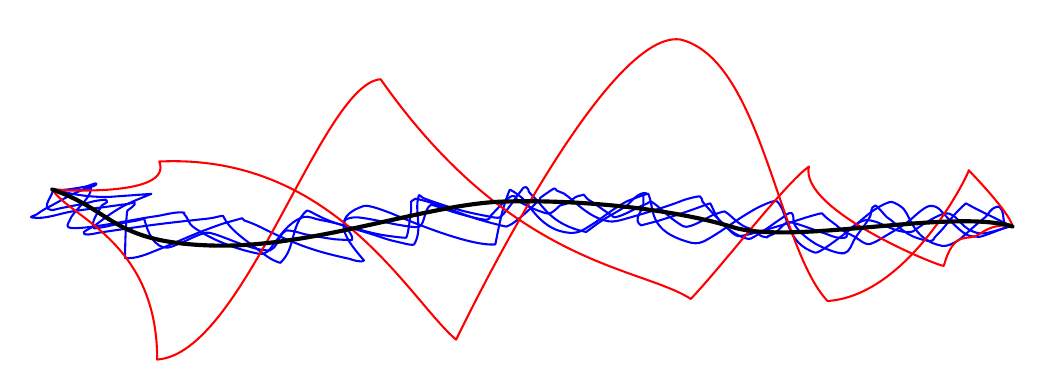
\begin{tikzpicture}[x=0.75pt,y=0.75pt,yscale=0.6,xscale=1]
\draw  [color=blue ,draw opacity=1 ][line width=0.75] [line join = round][line cap = round] (107.34,149.42) .. controls (109.06,146.87) and (101.14,134.38) .. (106.76,132.94) .. controls (107.11,132.85) and (107.64,132.8) .. (107.91,132.94) .. controls (112.34,135.2) and (122.31,137.36) .. (127.48,140) .. controls (127.98,140.26) and (133.04,141.42) .. (133.23,141.18) .. controls (135.22,138.64) and (131.53,138.04) .. (130.93,135.88) .. controls (129.52,130.84) and (125.58,123.07) .. (127.48,118.22) .. controls (127.65,117.79) and (134.21,119.92) .. (134.38,119.99) .. controls (138.36,121.62) and (143.31,123.15) .. (147.04,124.11) .. controls (148.03,124.36) and (151.64,125.9) .. (151.65,125.88) .. controls (152.63,120.35) and (154.61,106.12) .. (160.86,102.92) .. controls (163.74,101.45) and (167.35,105.48) .. (170.06,107.04) .. controls (172.09,108.21) and (179.81,115.44) .. (182.72,114.69) .. controls (188.91,113.11) and (204.42,99.17) .. (212.65,100.57) .. controls (213.01,100.63) and (212.37,101.02) .. (212.65,101.16) .. controls (216.01,102.88) and (216.15,112.39) .. (219.55,115.87) .. controls (219.72,116.05) and (219.21,116.37) .. (219.55,116.46) .. controls (222.04,117.09) and (226.67,114.58) .. (227.61,114.1) .. controls (230.69,112.53) and (241.69,109.74) .. (243.72,109.4) .. controls (244.2,109.31) and (251.72,108.59) .. (251.78,108.81) .. controls (253.35,114.84) and (241.64,125.13) .. (252.93,127.05) .. controls (256.35,127.64) and (270.8,121.89) .. (273.64,121.17) .. controls (274.56,120.93) and (282.57,118.43) .. (284,119.4) .. controls (286.96,121.42) and (286.46,133.69) .. (289.76,137.06) .. controls (290.19,137.5) and (295.5,134.12) .. (295.51,134.12) .. controls (300.17,131.26) and (309.59,126.69) .. (315.08,125.29) .. controls (318.74,124.35) and (318.06,127.51) .. (318.53,128.23) .. controls (320.01,130.5) and (326.77,143.58) .. (328.89,144.12) .. controls (331.13,144.69) and (331.03,141.42) .. (331.19,141.18) .. controls (332.77,138.76) and (341.07,131.73) .. (346.15,130) .. controls (347.97,129.37) and (351.46,135.79) .. (351.9,136.47) .. controls (352.08,136.73) and (352.57,136.93) .. (353.06,137.06) .. controls (357.58,138.22) and (357.3,143.44) .. (362.26,144.71) .. controls (362.88,144.87) and (363.41,145.3) .. (363.41,145.3) .. controls (363.41,145.3) and (365.04,141.87) .. (365.72,141.18) .. controls (369.07,137.74) and (373.76,131.77) .. (377.22,128.23) .. controls (377.61,127.84) and (377.61,126.86) .. (378.38,127.05) .. controls (382.78,128.18) and (389.87,135.87) .. (393.34,137.65) .. controls (393.78,137.87) and (395.64,140) .. (395.64,140) .. controls (395.64,140) and (398.17,137.3) .. (399.09,135.88) .. controls (402.56,130.55) and (406.26,125.02) .. (410.6,120.58) .. controls (410.73,120.45) and (411.98,119.24) .. (412.9,119.4) .. controls (417.06,120.11) and (423.18,127.19) .. (425.56,128.82) .. controls (425.76,128.96) and (430.95,132.14) .. (431.32,131.76) .. controls (435.81,127.17) and (437.23,121.09) .. (443.98,117.64) .. controls (447.04,116.07) and (447.09,112.13) .. (450.88,111.16) .. controls (452.93,110.64) and (451.52,111.49) .. (452.03,111.75) .. controls (457.56,114.58) and (457.69,119.3) .. (461.24,122.93) .. controls (461.58,123.28) and (462.86,123.11) .. (463.54,122.93) .. controls (465.86,122.34) and (476.52,115.71) .. (479.65,114.1) .. controls (481.02,113.41) and (485.29,109.66) .. (488.86,110.57) .. controls (491.29,111.19) and (489.57,113.32) .. (490.01,114.69) .. controls (490.62,116.57) and (495.71,124.1) .. (499.22,124.7) .. controls (505.46,125.76) and (512.18,114.14) .. (521.09,115.28) .. controls (521.61,115.35) and (522.07,115.61) .. (522.24,115.87) .. controls (523.86,118.36) and (533.69,129.1) .. (537.2,130) .. controls (537.89,130.17) and (538.96,130.27) .. (539.5,130) .. controls (544.76,127.3) and (545.43,116.41) .. (554.46,114.1) .. controls (558.17,113.16) and (569.42,120.86) .. (570,119.7) ;
\draw  [color=blue,draw opacity=1 ][line width=0.75] [line join = round][line cap = round] (107.34,149.42) .. controls (114.91,148.48) and (117.1,148.36) .. (122.57,149.06) .. controls (123.92,149.24) and (126.03,150.95) .. (126.03,150.24) .. controls (126.03,141.67) and (117.22,132.3) .. (115.67,124.34) .. controls (115.28,122.38) and (113.08,118.94) .. (116.82,118.46) .. controls (124.77,117.44) and (147.73,125.82) .. (157.1,127.88) .. controls (161.08,128.75) and (166.84,131.86) .. (170.91,130.82) .. controls (171.6,130.64) and (170.67,130.01) .. (170.91,129.64) .. controls (173.04,126.38) and (172.55,122.59) .. (175.51,119.05) .. controls (182.07,111.22) and (193.26,102.4) .. (206.59,97.86) .. controls (210.98,96.36) and (212.71,102.72) .. (213.49,104.33) .. controls (216.46,110.4) and (220.92,123.43) .. (228.46,127.29) .. controls (230.64,128.41) and (233.83,125.72) .. (236.51,124.93) .. controls (246.05,122.15) and (255.27,116.58) .. (265.29,113.16) .. controls (266.1,112.88) and (277.67,109.95) .. (277.95,110.81) .. controls (279.04,114.18) and (279.78,128.67) .. (280.25,132) .. controls (280.6,134.54) and (279.89,137.1) .. (280.25,139.65) .. controls (280.25,139.7) and (282.15,142.14) .. (282.55,142) .. controls (292.33,138.67) and (303.45,130.14) .. (312.47,125.52) .. controls (314.75,124.36) and (325.69,119.33) .. (326.28,119.64) .. controls (330.54,121.81) and (339.8,137.7) .. (342.4,141.41) .. controls (342.65,141.78) and (342.11,142.23) .. (342.4,142.59) .. controls (343.19,143.6) and (348.73,150.24) .. (349.3,150.24) .. controls (349.89,150.24) and (350.22,148.71) .. (350.45,148.48) .. controls (351.31,147.6) and (353.08,147.01) .. (353.9,146.12) .. controls (358.78,140.86) and (365.72,126.33) .. (375.77,123.76) .. controls (377.62,123.28) and (380.65,124.53) .. (381.53,124.93) .. controls (390.97,129.28) and (404.44,136.04) .. (411.45,140.82) .. controls (412.02,141.21) and (418.4,144.33) .. (419.51,143.77) .. controls (420.49,143.26) and (420.36,140.26) .. (420.66,139.65) .. controls (423.43,133.98) and (427.14,127.35) .. (431.01,121.4) .. controls (431.78,120.23) and (435.35,112.42) .. (437.92,111.98) .. controls (441.24,111.42) and (464.99,123.88) .. (468.99,126.11) .. controls (469.91,126.62) and (477.97,130.7) .. (478.2,130.23) .. controls (480.1,126.34) and (483.88,122.7) .. (486.26,119.05) .. controls (487.8,116.69) and (489.02,115.2) .. (492.01,113.16) .. controls (495.19,111) and (496.55,107.31) .. (500.07,105.51) .. controls (501.7,104.67) and (506.6,109.83) .. (506.97,110.22) .. controls (512.77,116.15) and (517.87,120.45) .. (521.94,126.7) .. controls (523.15,128.56) and (527.72,135.53) .. (529.99,136.12) .. controls (534.16,137.18) and (536.61,130.08) .. (536.9,129.64) .. controls (539.65,125.41) and (545.07,114.28) .. (549.56,111.98) .. controls (549.73,111.89) and (553.72,111.28) .. (554.16,111.4) .. controls (556.53,112) and (566.13,118.7) .. (567.97,119.64) .. controls (569.29,120.31) and (568.03,121.99) .. (570,119.7) ;
\draw [color=blue,draw opacity=1 ][line width=0.75] [line join = round][line cap = round]   (107.34,149.42) .. controls (111.43,147.84) and (119.65,150.67) .. (122.88,151.53) .. controls (125.07,152.12) and (128.63,155.31) .. (128.63,153.99) .. controls (128.63,152.6) and (126.67,151.72) .. (125.18,150.92) .. controls (116.37,146.21) and (111.21,139.9) .. (104.46,134.3) .. controls (102.6,132.76) and (101.39,131.02) .. (99.86,129.38) .. controls (99.09,128.56) and (96.02,127.33) .. (97.56,126.92) .. controls (104,125.2) and (110.64,130.16) .. (117.12,131.84) .. controls (124.24,133.69) and (131.8,135) .. (138.99,136.76) .. controls (141.33,137.34) and (144.07,137.64) .. (145.89,138.61) .. controls (146.28,138.81) and (146.87,139.5) .. (147.04,139.22) .. controls (148.26,137.27) and (143.98,133.28) .. (143.59,132.46) .. controls (143.13,131.46) and (142.44,109.4) .. (142.44,94.31) .. controls (148.02,93.45) and (154.26,98.39) .. (157.4,100.46) .. controls (169.39,108.35) and (175.9,114.22) .. (189.63,122) .. controls (190.64,122.57) and (198.83,126.3) .. (198.83,126.3) .. controls (198.83,126.3) and (199.87,124.52) .. (199.99,124.46) .. controls (201.96,123.4) and (205.42,121.16) .. (208.04,118.92) .. controls (214.66,113.26) and (224.37,105.88) .. (233.36,101.08) .. controls (238.57,98.29) and (244.49,95.88) .. (250.63,93.69) .. controls (250.85,93.61) and (256.31,90.01) .. (257.53,92.46) .. controls (249.47,108.22) and (240.13,126.85) .. (257.53,136.15) .. controls (259.87,137.4) and (268.21,131.71) .. (270.19,130.61) .. controls (271.26,130.02) and (306.85,103.41) .. (320.83,105.28) .. controls (323.13,124.7) and (324.28,134.7) .. (327.74,149.07) .. controls (328.49,149.48) and (333.19,143.37) .. (333.49,142.92) .. controls (337.84,136.41) and (343.14,116.4) .. (356.51,114.61) .. controls (361.38,113.96) and (363.98,117.8) .. (365.72,119.53) .. controls (372.54,126.37) and (376.68,133.2) .. (384.13,139.84) .. controls (384.72,140.37) and (394.38,146.38) .. (394.49,145.99) .. controls (397.89,133.27) and (393.69,116.03) .. (415.2,106.61) .. controls (418.23,105.29) and (420.97,107.41) .. (422.11,108.46) .. controls (429.85,115.6) and (435.53,123.33) .. (442.83,130.61) .. controls (444.94,132.72) and (447.05,134.85) .. (449.73,136.76) .. controls (451.53,138.05) and (455.78,141.37) .. (456.64,139.84) .. controls (462.35,129.66) and (460.41,106.44) .. (475.05,98.61) .. controls (476.89,97.63) and (490.97,116.21) .. (491.16,116.46) .. controls (496.74,123.41) and (502.81,134.99) .. (510.73,139.22) .. controls (513.02,140.45) and (517.32,134.36) .. (517.63,133.69) .. controls (521.11,126.26) and (522.83,108.39) .. (536.05,104.15) .. controls (539.37,103.09) and (544.52,109.23) .. (545.26,110.31) .. controls (549.09,115.94) and (552.42,121.4) .. (556.76,126.92) .. controls (558.98,129.73) and (558.49,133.38) .. (562.52,135.53) .. controls (562.79,135.68) and (563.55,135.73) .. (563.67,135.53) .. controls (566.03,131.74) and (565.27,127.37) .. (565.97,123.23) .. controls (566.25,121.58) and (567.12,119.96) .. (570,119.7) ;
\draw  [color=blue,draw opacity=1 ][line width=0.75] [line join = round][line cap = round] (107.34,149.42) .. controls (120.31,144.12) and (127.71,143.06) .. (135.54,143.53) .. controls (136.49,143.59) and (155.1,145.89) .. (155.1,145.89) .. controls (155.1,145.89) and (150.5,142.75) .. (148.2,141.18) .. controls (138.43,134.52) and (133.66,127.57) .. (127.48,119.99) .. controls (126.76,119.1) and (120.53,114.71) .. (122.88,113.52) .. controls (124.9,112.48) and (128.74,114.44) .. (129.78,114.69) .. controls (154.53,120.8) and (158.04,121.66) .. (181.57,125.88) .. controls (184.14,126.33) and (186.17,127.05) .. (187.33,127.64) .. controls (187.33,127.64) and (189.58,128.4) .. (189.63,128.23) .. controls (192.62,117.53) and (199.23,110.36) .. (206.89,100.57) .. controls (209.4,97.36) and (212.79,92.84) .. (216.1,91.15) .. controls (216.48,90.95) and (217.08,90.3) .. (217.25,90.56) .. controls (224.91,102.32) and (221.7,119.76) .. (229.91,132.35) .. controls (230.25,132.87) and (232.19,131.19) .. (232.21,131.17) .. controls (234.73,128.96) and (237.2,126.72) .. (240.27,124.7) .. controls (247.73,119.79) and (257.64,115.74) .. (265.59,111.16) .. controls (270.91,108.1) and (271.48,108.28) .. (275.95,106.45) .. controls (277.56,105.79) and (281.33,104.24) .. (281.7,105.28) .. controls (286.25,118.07) and (281.47,131.74) .. (284,144.71) .. controls (284.17,145.58) and (285.2,143.03) .. (286.3,142.36) .. controls (291.69,139.05) and (297.38,135.86) .. (303.57,132.94) .. controls (307.4,131.13) and (311.8,129.64) .. (316.23,128.23) .. controls (318.28,127.57) and (322.36,125.88) .. (323.13,127.05) .. controls (327.35,133.53) and (330.12,142.22) .. (333.49,148.83) .. controls (333.56,148.97) and (334.31,151.94) .. (335.79,151.18) .. controls (337.05,150.54) and (336.61,148.39) .. (336.94,147.65) .. controls (338.22,144.87) and (340.14,142.18) .. (341.55,139.41) .. controls (345.66,131.35) and (350.65,120.03) .. (364.56,115.28) .. controls (364.63,115.26) and (369.6,121.48) .. (370.32,122.34) .. controls (374.25,127.03) and (379.95,131.66) .. (384.13,136.47) .. controls (385.6,138.16) and (388.66,145.57) .. (392.19,146.48) .. controls (392.53,146.56) and (393.07,146.61) .. (393.34,146.48) .. controls (394.32,145.97) and (392.21,145.51) .. (392.19,145.3) .. controls (391.83,142.56) and (392.47,139.8) .. (392.19,137.06) .. controls (391.72,132.58) and (386.88,124.83) .. (391.04,120.58) .. controls (391.06,120.55) and (399.03,124.08) .. (399.09,124.11) .. controls (403.66,126.45) and (411.72,130.76) .. (416.35,133.53) .. controls (420.37,135.92) and (424.33,138.49) .. (424.41,138.24) .. controls (427.05,130.13) and (426.81,125.4) .. (433.62,117.05) .. controls (434.94,115.43) and (436.32,113.8) .. (438.22,112.34) .. controls (439.58,111.29) and (442.76,108.89) .. (443.98,109.98) .. controls (449.64,115.05) and (454.05,121.15) .. (458.94,126.46) .. controls (459.82,127.42) and (460.21,128.49) .. (461.24,129.41) .. controls (461.78,129.89) and (463.06,131.08) .. (463.54,130.58) .. controls (464.83,129.26) and (464.29,123.98) .. (464.69,122.34) .. controls (466.02,116.89) and (470.5,110.52) .. (475.05,105.86) .. controls (476.38,104.51) and (485.17,97.27) .. (488.86,98.21) .. controls (491.5,98.89) and (492.83,106.26) .. (493.47,108.22) .. controls (495.6,114.77) and (499.71,121.76) .. (501.52,128.23) .. controls (502.14,130.43) and (501.41,135.24) .. (503.82,136.47) .. controls (504.67,136.9) and (508.8,127.85) .. (509.58,127.05) .. controls (515,121.51) and (517.12,111.91) .. (529.14,108.22) .. controls (532.25,107.26) and (532.04,110.24) .. (532.6,111.16) .. controls (534.26,113.89) and (535.84,116.63) .. (537.2,119.4) .. controls (540.3,125.74) and (543.16,132.06) .. (547.56,138.24) .. controls (547.62,138.32) and (551.56,134.61) .. (552.16,134.12) .. controls (552.17,134.1) and (569.42,119.87) .. (570,119.7) ;
\draw [color=red,draw opacity=1 ][line width=0.75] [line join = round][line cap = round]   (107.34,149.42) .. controls (115.7,127.07) and (158,107.5) .. (157.91,12.84) .. controls (200,17.5) and (237,234.5) .. (265.58,237.92) .. controls (329,87.5) and (391,87.5) .. (415,61.5) .. controls (432,91.5) and (459.41,152.34) .. (471.91,167.84) .. controls (467,132.5) and (536.41,86.34) .. (536.91,88.09) .. controls (542,118.5) and (548.52,106.92) .. (554,113.5) .. controls (559.48,120.08) and (564.91,121.63) .. (570,119.7) ;
\draw [color=red,draw opacity=1 ][line width=0.75] [line join = round][line cap = round]   (107.34,149.42) .. controls (108.91,149.09) and (166,142.5) .. (158.91,171.84) .. controls (243,178.5) and (279,61.5) .. (301.91,28.84) .. controls (302.33,29.33) and (373,278.5) .. (409.91,269.84) .. controls (449,254.5) and (457,101.5) .. (480.91,59.84) .. controls (521,64.5) and (549.67,164.67) .. (548.91,164.84) .. controls (549,164.67) and (569.09,130.36) .. (570,119.7) ;
\draw [color=black,line width=1.5][line cap = round]    (107.34,149.42) .. controls (137.26,132.06) and (136.11,106.75) .. (184.45,104.39) .. controls (232.79,102.04) and (288.03,137.94) .. (324.86,139.71) .. controls (361.69,141.47) and (406.57,133.82) .. (435.34,119.11) .. controls (464.12,104.39) and (541.23,134.41) .. (570,119.7) ;
\end{tikzpicture}
\caption{The black line corresponds to the classical solution, $\phicl$. The blue lines describes the configurations which sum up coherently in the path integral, whereas red lines represent those configurations whose contributions to the path integral is suppressed by $Q(\chi)$ since they strongly deviate from the classical solution.}
\label{fig:paths-localized-classical-solution}
\end{figure}

Notice that if such approximation holds, the soliton can be analized as a (extended) quantum mechanical particle localized around the classical solution. However, in order to give a complete QFT description, we should improve our description, in such a way that we are able to describe creation and annihilation of solitons. 

\skipline

Notice that in general each of the dominant classical configurations (blue lines in fig.~\ref{fig:paths-localized-classical-solution}) will not be associated to a specific solution of the equations of motion, because in different regions in the Euclidean space-time the field may be close to different local minima of the action, and we need to interpolate among them. For example, in our $\phi^4$ model in some regions $\phi$ may be close to the absolute minima $\phi_+$, in some other to the kink solution $\phi^S$. 

In order to take into account this issue, we wish to find a set of classical configurations $\{\phi_i\}_{i\in I}$ and a partition $\{\consp_i\}_{i\in I}$ of the space $\consp$ of all configurations of $\phi$,\footnote{The space $\consp$ is very singular, for example in $\phi_2^4$ it may be $\schw'(\R^2)$.} with $\phi_i\in\consp_i$, such that\todo{Qui ho fatto delle modifiche poiché, se non vado errato, nella versione data in classe non veniva risolto il problema di configurazioni che interpolano tra più minimi dell'azione.}
\begin{enumerate}[label=(\arabic*), start=0]
	\item for each $\phi\in\consp$ and $i\in I$, expanding $\phi=\phi_i+\chi_i$ we can rewrite
	\begin{eq}
		S(\phi)=S(\phi_i)+Q_i(\chi_i)+R_i(\chi_i)
	\end{eq}
	with $Q_i(\chi_i)$ containing terms up to the second order in $\chi_i$ and $R_i(\chi_i)$ containing terms of higher order;
	\item if $\phi\in\consp_i$ then $\vert e^{-R_i(\phi)}-1\vert\ll1$;
	\item if $\phi\not\in\consp_i$ then $e^{-Q_i(\phi)}\ll1$ (i.e. $\phi$ strongly deviate from $\phi_i^\tcl$);
	\item $\bigcup_i\consp_i$ is the configuration space of $\phi$;
	\item $\consp_i\cap\consp_j=\emptyset$ for $i\neq j$.
\end{enumerate}
One should think at $\{\phi_i\}_{i\in I}$ as the union of all the classical solutions of equations of motion (vacuum configurations and local minima of the action) together with a set of ``inequivalent'' configurations which interpolate between different classical solutions. The meaning of ``inequivalent'' is specified by the above conditions. For instance, there may be a configuration $\phi_i$ which coincide with $\phi^S_+$ up to $x_0$ and coincide with $\phi^S_-$ for $x$ greater than $x_0$. Then using (1) and (2) we see that $R_i(\phi)$ is very close to zero if $\phi$ is close to $\phi_i$, and $e^{Q_i(\phi)}$ is almost zero if $\phi$ strongly deviates from $\phi_i$. The five properties together ensures that there are no other configurations $\phi_j\not\in\consp_i$ which are a slight deformation of $\phi_i$. 

According to (3) and (4) we can defined a partition of unity
\begin{eq}
	1_\consp=\sum_i X_i(\phi)
	\twith
	X_i(\phi)=\begin{cases}
		1\tif\phi\in\consp_i\\
		0\tif\phi\not\in\consp_i
	\end{cases}
\end{eq}
which can be inserted in the path integral obtaining an ``improved semi-classical approximation'':\footnote{Here we denote by $\int_{\consp_i-\phi}\pide\chi$ the integration over those configurations $\chi$ such that $\phi+\chi\in\consp_i$. The last step follows easily since $\consp$ contain all the possible configurations, hence $\consp-\phi=\consp$ for any $\phi$.}
\begin{eq}\label{eq:improv-semiclass-approx}
	\int_\consp\pide\phi\,e^{-S(\phi)}F(\phi)
	&=\sum_{i\in I}\int_\consp\pide\phi\,e^{-S(\phi)}F(\phi)X_i(\phi)\\
	&=\sum_{i\in I}\int_{\consp_i}\!\pide\phi\,e^{-S(\phi)}F(\phi)\\
	&=\sum_{i\in I}\int_{\consp_i-\phi_i}\!\!\!\pide\chi_i\,e^{-S(\phi_i)-Q_i(\chi_i)-R_i(\chi_i)}F(\phi_i+\chi_i)\\
	&\overset{(1)}{\approx}\sum_{i\in I}e^{-S(\phi_i)}\int_{\consp_i-\phi_i}\!\!\!\pide\chi_i\,e^{-Q_i(\chi_i)}F(\phi_i+\chi_i)\\
	&\overset{(2)}{\approx}\sum_{i\in I}e^{-S(\phi_i)}\int_{\consp-\phi_i}\!\!\!\pide\chi_i\,e^{-Q_i(\chi_i)}F(\phi_i+\chi_i)\\
	&=\sum_{i\in I}e^{-S(\phi_i)}\int_{\consp}\!\pide\chi_i\,e^{-Q_i(\chi_i)}F(\phi_i+\chi_i)\\
\end{eq}
Hence such approximation considers fluctuations around various possible local minima of the action, neglecting higher order contributions coming from the various $R_i(\chi_i)$'s. 

\subsubsection{Defects in QFT}

For a fixed configuration $\phi$ let $\Gamma$ be a region in the Euclidean space-time where the $\phi$ deviates strongly from the global minimum of the action (i.e. from the vacuum) but it is close to a local minimum (usually corresponding to a classical solution of the equations of motion). 
If $\Gamma$ is connected it is said to be the support of a \emph{defect}.\footnote{The notion of defect comes from the study of crystals: a defect is an irregularity of the structure. Such irregularities usually create new energy levels, which have higher energy with respect to the ground state. Similarly, in QFT the notion of defect has been adapted, describing local minima of the action, disjointed from the global ones (the vacua).} 
If the Euclidean space-time minus the support of the defect $\Gamma$ is contractible to the Euclidean space-time minus a $n$-dimensional manifold, then we call the defect a $n$-dimensional defect. In particular we can have a point defect, a line defect, etc. In mathematical language, $\Gamma$ is a point/line/surface/\ldots/n-dimensional defect if it is the tubular neighbourhood of a point/line/surface/\ldots/n-dimensional manifold. 

In high energy language, sometimes one also use the word \emph{$p$-brane} for a $(p+1)$-dimensional defect, although often this terminology is deserved to cases in which the defect is strictly $(p+1)$-dimensional (without contracting its complement). 

Notice that free theories has only one minimum, therefore in order to have defects we should consider interacting theories.

\skipline

For our $\phi_2^4$ theory the kink is a line defect. Indeed $\Gamma$ appears in the partition function when the field $\phi$ changes sign around a bounded region. The line where $\phi$ vanishes is called the \emph{locus of the defect} and is clearly a closed line. An example is shown in fig.~\ref{fig:defect}. 

\begin{figure}[h]
\centering
\begin{tikzpicture}[x=0.75pt,y=0.75pt,yscale=-0.7,xscale=0.7]
\draw  [color=blue ,draw opacity=0.7 ][line width=6]  (197,110) .. controls (217,100) and (307,90) .. (287,110) .. controls (267,130) and (267,140) .. (287,170) .. controls (307,200) and (217,200) .. (197,170) .. controls (177,140) and (177,120) .. (197,110) -- cycle ;
\draw  [color=black][line width=1] (197,110) .. controls (217,100) and (307,90) .. (287,110) .. controls (267,130) and (267,140) .. (287,170) .. controls (307,200) and (217,200) .. (197,170) .. controls (177,140) and (177,120) .. (197,110) -- cycle ;
\draw   (127,50.33) -- (379.33,50.33) -- (356,220) -- (103.67,220) -- cycle ;
\draw (234.67,130.07) node [anchor=north]   {$\phi< 0$};
\draw (325.33,60.73) node [anchor=north]    {$\phi>0$};
\draw (300,130) node [anchor=north][color=darkblue]   {$\Gamma$};
\end{tikzpicture}
\caption{The defect $\Gamma$ is represented by the blue thick line. The black line correspond to the locus of the defect, i.e. where $\phi=0$.}
\label{fig:defect}
\end{figure}

For the classical kink discussed before in the quantum mechanical treatment, the locus of the defect is time independent and is parametrized by the modulus of the kink. A typical configuration of $\phi$ far away from the locus of the defect should be close to one of the two global minima $\phi_\pm$. Instead near the region $\phi=0$ typical configurations should be close to a kink, in order to maintain $S(\phi)$ close to a (local) minimum. 

If the vacuum expectation value is positive, $\langle\phi\rangle>0$, which can be achieved by imposing $\phi_+$ boundary conditions at $\infty$, the situation is the one represented in fig.~\ref{fig:defects-positive-boundaries-conditions}. 

\begin{figure}[h]
\centering
\tikzset{every picture/.style={line width=0.75pt}}  
\begin{tikzpicture}[x=0.75pt,y=0.75pt,yscale=-1,xscale=1]

\draw    [color=blue ,draw opacity=0.7 ][line width=6] (130,170) .. controls (150,160) and (240,150) .. (220,170) .. controls (200,190) and (200,200) .. (220,230) .. controls (240,260) and (150,260) .. (130,230) .. controls (110,200) and (110,180) .. (130,170) -- cycle ;
\draw    [color=blue ,draw opacity=0.7 ][line width=6] (427.33,161) .. controls (449,131) and (451.67,158) .. (471,168) .. controls (490.33,178) and (514,181.67) .. (487.67,205.67) .. controls (461.33,229.67) and (447.33,251) .. (427.33,221) .. controls (407.33,191) and (405.67,191) .. (427.33,161) -- cycle ;
\draw    [color=blue ,draw opacity=0.7 ][line width=6] (360.33,123.33) .. controls (380.33,113.33) and (400.67,105) .. (450.33,123.33) .. controls (500,141.67) and (582,179.67) .. (534.67,233.67) .. controls (487.33,287.67) and (333.33,234.33) .. (306.67,207.67) .. controls (280,181) and (340.33,133.33) .. (360.33,123.33) -- cycle ;
\draw   [color=black][line width=1] (130,170) .. controls (150,160) and (240,150) .. (220,170) .. controls (200,190) and (200,200) .. (220,230) .. controls (240,260) and (150,260) .. (130,230) .. controls (110,200) and (110,180) .. (130,170) -- cycle ;
\draw   [color=black][line width=1] (427.33,161) .. controls (449,131) and (451.67,158) .. (471,168) .. controls (490.33,178) and (514,181.67) .. (487.67,205.67) .. controls (461.33,229.67) and (447.33,251) .. (427.33,221) .. controls (407.33,191) and (405.67,191) .. (427.33,161) -- cycle ;
\draw   [color=black][line width=1] (360.33,123.33) .. controls (380.33,113.33) and (400.67,105) .. (450.33,123.33) .. controls (500,141.67) and (582,179.67) .. (534.67,233.67) .. controls (487.33,287.67) and (333.33,234.33) .. (306.67,207.67) .. controls (280,181) and (340.33,133.33) .. (360.33,123.33) -- cycle ;

\draw    (85.67,78.67) -- (567.67,78.67) -- (567.67,278.67) -- (85.67,278.67) -- cycle ;

\draw (89.67,64) node [anchor=north west][inner sep=0.75pt]    {$+$};
\draw (157.31,64) node [anchor=north west][inner sep=0.75pt]    {$+$};
\draw (225.07,64) node [anchor=north west][inner sep=0.75pt]    {$+$};
\draw (292.77,64) node [anchor=north west][inner sep=0.75pt]    {$+$};
\draw (360.47,64) node [anchor=north west][inner sep=0.75pt]    {$+$};
\draw (428.17,64) node [anchor=north west][inner sep=0.75pt]    {$+$};
\draw (495.87,64) node [anchor=north west][inner sep=0.75pt]    {$+$};
\draw (563.57,64) node [anchor=north west][inner sep=0.75pt]    {$+$};

\draw (89.67,281.4) node [anchor=north west][inner sep=0.75pt]    {$+$};
\draw (157.31,281.4) node [anchor=north west][inner sep=0.75pt]    {$+$};
\draw (225.07,281.4) node [anchor=north west][inner sep=0.75pt]    {$+$};
\draw (292.77,281.4) node [anchor=north west][inner sep=0.75pt]    {$+$};
\draw (360.47,281.4) node [anchor=north west][inner sep=0.75pt]    {$+$};
\draw (428.17,281.4) node [anchor=north west][inner sep=0.75pt]    {$+$};
\draw (495.87,281.4) node [anchor=north west][inner sep=0.75pt]    {$+$};
\draw (563.57,281.4) node [anchor=north west][inner sep=0.75pt]    {$+$};

\draw (70,274.67) node [anchor= west][inner sep=0.75pt]    {$+$};
\draw (70,226.67) node [anchor= west][inner sep=0.75pt]    {$+$};
\draw (70,178.67) node [anchor= west][inner sep=0.75pt]    {$+$};
\draw (70,130.67) node [anchor= west][inner sep=0.75pt]    {$+$};
\draw (70,82.67) node [anchor= west][inner sep=0.75pt]    {$+$};

\draw (574,274.67) node [anchor= west][inner sep=0.75pt]    {$+$};
\draw (574,226.67) node [anchor= west][inner sep=0.75pt]    {$+$};
\draw (574,178.67) node [anchor= west][inner sep=0.75pt]    {$+$};
\draw (574,130.67) node [anchor= west][inner sep=0.75pt]    {$+$};
\draw (574,82.67) node [anchor= west][inner sep=0.75pt]    {$+$};

\draw (145.33,194.4) node [anchor=north west] {$\phi < 0$};
\draw (335.67,181.07) node [anchor=north west] {$\phi < 0$};
\draw (144,103.07) node [anchor=north west] {$\phi  >0$};
\draw (432,183.07) node [anchor=north west] {$\phi  >0$};
\draw (115,239.73) node [anchor=north west][color=darkblue] {$\Gamma _{1}$};
\draw (338.67,237.4) node [anchor=north west][color=darkblue] {$\Gamma _{2}$};
\draw (400,147) node [anchor=north west][color=darkblue] {$\Gamma _{3}$};

\end{tikzpicture}
\caption{Defects (blue lines) and their locus (black lines) in presence of $\langle\phi\rangle>0$ boundary conditions, in the finite volume regularization.}
\label{fig:defects-positive-boundaries-conditions}
\end{figure}

In the lattice approximation (replacing $\phi^4$ by the Ising model) such defects are called \emph{Peierls contours}. 

\skipline

\todo{Qui ho un po reinterpretato perché non riuscivo a capire come $S(\Gamma_1,\ldots,\Gamma_N)$ fosse definito a partire dai defects, che sono regioni dello spazio tempo.}
Let us consider again eq.~\eqref{eq:improv-semiclass-approx}. Notice that to each $\consp_i$ we can associate the defects $\Gamma_{i,1},\ldots,\Gamma_{i,n}$ appearing in the configurations $\phi\in\consp_i$. Then, we can consider 
\begin{eq}
	\int_{\consp_i-\phi_i}\pide\chi_i\,e^{-S(\phi_i)-Q_i(\chi_i)}
\end{eq}
as a Boltzmann weight of the \emph{gas of defects} $\{\Gamma_{i,1},\ldots,\Gamma_{i,N}\}$ appearing in the configurations of $\consp_i$. From such Boltzmann weight, we can define the action associated with the gas:
\begin{eq}
	S(\Gamma_{i,1},\ldots,\Gamma_{i,N})
\end{eq}
Similarly, we can define $S(\Gamma)$ by computing $\int\pide\phi\,e^{-S(\phi)}$ over all the configurations with support contained in $\Gamma$. 
Notice that the same defect $\Gamma$ can be associated to different sets $\consp_j$, as in general classical configurations may interpolate between several local minima of the action, but each gas of defects $\{\Gamma_1,\ldots,\Gamma_N\}$ is uniquely associated to some $\consp_i$, for the same reasons which lead us to eq.~\eqref{eq:improv-semiclass-approx}. 

We can now define the interaction between defects in the gas $\{\Gamma_1,\ldots,\Gamma_N\}$ as
\begin{eq}
	V(\Gamma_1,\ldots,\Gamma_N):=S(\Gamma_1,\ldots,\Gamma_N)-\sum_{k=1}^NS(\Gamma_k)
\end{eq}
One should notice that if the defects are separated enough each other, so that no configuration with non-zero measure interpolate between them, then $V(\Gamma_1,\ldots,\Gamma_N)=0$ and the defects do not interact among each other. 

Finally, neglecting contributions coming from fluctuations around the vacuum, we get that in the ``improved semi-classical approximation'' the partition function of the system can be expressed as\todo{Qui ho modificato la formula data a lezione al fine di evitare di contare più volte il contributo dello stesso gas di defects.}
\begin{eq}
	\int_\consp\pide\phi\,e^{-S(\phi)}
	&\approx\sum_{i\in I}e^{\displaystyle-S(\Gamma_{i,1},\ldots,\Gamma_{i,N})}\\
	&=\sum_{i\in I}\underbrace{\prod_{k=1}^Ne^{\displaystyle-S(\Gamma_{i,k})}}_{\text{Non-interacting}\atop\text{gas of defects}}\,\underbrace{\vphantom{\prod_{k}}e^{\displaystyle-V(\Gamma_{i,1},\ldots,\Gamma_{i,N})}}_{\text{Interactions}\atop\text{among defects}}
\end{eq}
which can be interpreted as a partition function of the interacting gas of defects, which by construction have closed locus. \todo{Qui ho un dubbio che è legato ad un'altra domanda che le ho fatto più sotto. Immagino che questa interazione tra defects risulta poi essere un'interazione tra kinks. Ha senso questo visto che kinks dovrebbero esser configurazioni solitarie (perlomeno a livello classico)? In tal caso, è possibile definire un'azione interagente per kink in QFT che tenga conto di questo tipo di interazioni?}

\skipline

In the lattice line defects are close contours in the dual lattice, between sites in which the field $\phi$ has opposite sign, as shown in fig.~\ref{fig:defect-lattice-1} and fig.~\ref{fig:defect-lattice-2}. 

\begin{figure}[H]
\centering
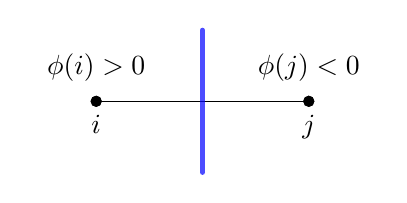
\begin{tikzpicture}[xscale=0.9,yscale=0.9]
\draw (0,0) -- (3,0);
\draw [color=blue ,draw opacity=0.7, line width=2, line cap = round](1.5,-1) -- (1.5,1);
\draw (0,0) circle (2pt) node [anchor=south][inner sep=7pt]    {$\phi(i)>0$};
\draw (0,0) circle (2pt)[fill=black] node [anchor=north][inner sep=5pt]    {$i$};
\draw (3,0) circle (2pt) node [anchor=south][inner sep=7pt]    {$\phi(j)<0$};
\draw (3,0) circle (2pt)[fill=black] node [anchor=north][inner sep=5pt]    {$j$};
\end{tikzpicture}
\caption{The elementary component (blue line) of a defect. Given a link in the lattice between two sites where $\phi$ has opposite sign, the defect is made by considering the orthogonal link in the dual lattice.}
\label{fig:defect-lattice-1}
\end{figure}

\begin{figure}[h]
\centering
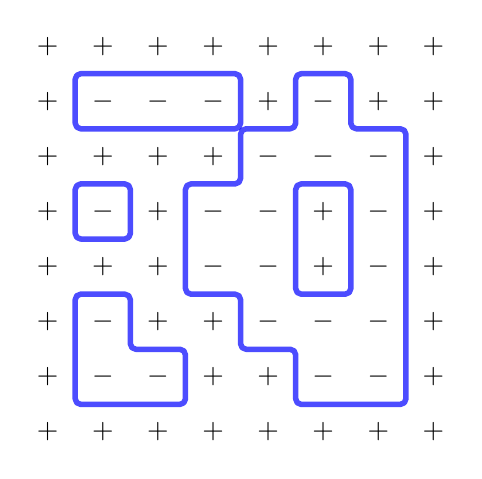
\begin{tikzpicture}[xscale=0.7,yscale=0.7]
\draw [color=blue ,draw opacity=0.7, line width=2, line cap = round, line join = round, rounded corners=2pt] (1.5,6.5) -- (4.5,6.5) -- (4.5,7.5) -- (1.5,7.5) -- cycle;
\draw [color=blue ,draw opacity=0.7, line width=2, line cap = round, line join = round, rounded corners=2pt] (1.5,4.5) -- (2.5,4.5) -- (2.5,5.5) -- (1.5,5.5) -- cycle;
\draw [color=blue ,draw opacity=0.7, line width=2, line cap = round, line join = round, rounded corners=2pt] (1.5,1.5) -- (3.5,1.5) -- (3.5,2.5) -- (2.5,2.5) -- (2.5,3.5) -- (1.5,3.5) -- cycle;
\draw [color=blue ,draw opacity=0.7, line width=2, line cap = round, line join = round, rounded corners=2pt] (5.5,1.5) -- (7.5,1.5) -- (7.5,6.5) -- (6.5,6.5) -- (6.5,7.5) -- (5.5,7.5) -- (5.5,6.5) -- (4.5,6.5) -- (4.5,5.5) -- (3.5,5.5) -- (3.5,3.5) -- (4.5,3.5) -- (4.5,2.5) -- (5.5,2.5) -- cycle;
\draw [color=blue ,draw opacity=0.7, line width=2, line cap = round, line join = round, rounded corners=2pt] (5.5,5.5) -- (6.5,5.5) -- (6.5,3.5) -- (5.5,3.5) -- cycle;
\draw(1,1) node {$+$};\draw(2,1) node {$+$};\draw(3,1) node {$+$};\draw(4,1) node {$+$};\draw(5,1) node {$+$};\draw(6,1) node {$+$};\draw(7,1) node {$+$};\draw(8,1) node {$+$};
\draw(1,2) node {$+$};\draw(2,2) node {$-$};\draw(3,2) node {$-$};\draw(4,2) node {$+$};\draw(5,2) node {$+$};\draw(6,2) node {$-$};\draw(7,2) node {$-$};\draw(8,2) node {$+$};
\draw(1,3) node {$+$};\draw(2,3) node {$-$};\draw(3,3) node {$+$};\draw(4,3) node {$+$};\draw(5,3) node {$-$};\draw(6,3) node {$-$};\draw(7,3) node {$-$};\draw(8,3) node {$+$};
\draw(1,4) node {$+$};\draw(2,4) node {$+$};\draw(3,4) node {$+$};\draw(4,4) node {$-$};\draw(5,4) node {$-$};\draw(6,4) node {$+$};\draw(7,4) node {$-$};\draw(8,4) node {$+$};
\draw(1,5) node {$+$};\draw(2,5) node {$-$};\draw(3,5) node {$+$};\draw(4,5) node {$-$};\draw(5,5) node {$-$};\draw(6,5) node {$+$};\draw(7,5) node {$-$};\draw(8,5) node {$+$};
\draw(1,6) node {$+$};\draw(2,6) node {$+$};\draw(3,6) node {$+$};\draw(4,6) node {$+$};\draw(5,6) node {$-$};\draw(6,6) node {$-$};\draw(7,6) node {$-$};\draw(8,6) node {$+$};
\draw(1,7) node {$+$};\draw(2,7) node {$-$};\draw(3,7) node {$-$};\draw(4,7) node {$-$};\draw(5,7) node {$+$};\draw(6,7) node {$-$};\draw(7,7) node {$+$};\draw(8,7) node {$+$};
\draw(1,8) node {$+$};\draw(2,8) node {$+$};\draw(3,8) node {$+$};\draw(4,8) node {$+$};\draw(5,8) node {$+$};\draw(6,8) node {$+$};\draw(7,8) node {$+$};\draw(8,8) node {$+$};
\end{tikzpicture}
\caption{The loci of the lattice are denoted by $+$ and $-$ depending on wether the field has positive or negative value on them. The blue lines represent defects which are supported in the dual lattice and are constructed according to fig.~\ref{fig:defect-lattice-1}.}
\label{fig:defect-lattice-2}
\end{figure}

\subsubsection{Particle-antiparticle virtual pairs}

Since the support of line defects locally looks like the world line of a particle, closed loops naturally correspond to particle-antiparticle virtual pairs.

\tikzset{every picture/.style={line width=0.75pt}}   
\begin{figure}[H]
\centering
\tikzstyle{arrow} = [thick,->,>=stealth]
\begin{tikzpicture}[x=0.75pt,y=0.75pt,yscale=-0.8,xscale=0.8]
\draw  [arrow]  (101,202) -- (101,85) ;
\draw    (190.5,191) .. controls (160.91,171.11) and (160.97,113.12) .. (186.1,93.69) ;
\draw [shift={(188.5,92)}, rotate = 507.53] [fill=black  ][line width=0.08]  (8.93,-4.29) -- (0,0) -- (8.93,4.29) -- cycle    ;
\draw    (188.5,92) .. controls (219.21,109.06) and (219.98,166.53) .. (192.66,189.32) ;
\draw [shift={(190.5,191)}, rotate = 324] [fill=black  ][line width=0.08] (8.93,-4.29) -- (0,0) -- (8.93,4.29) -- cycle    ;
\draw (143.5,172) node [anchor=north west][inner sep=0.75pt]  [rotate=90] [align=left] {particle};
\draw (235.5,99) node [anchor=north west][inner sep=0.75pt]  [rotate=-90] [align=left] {antiparticle};
\draw (80,90) node [anchor=north west][inner sep=0.75pt]    {$\tau $};
\end{tikzpicture}
\end{figure}

A natural question is then how to construct quantum field operators creating and annihilating particles giving rise to the defects, as quantum particles. We first show that the Euclidean two-points function of a free massive scalar field\footnote{The object $(-\Delta+m^2)^{-1}(x,y)$ is the kernel of the operator $(-\Delta+m^2)^{-1}$. If you are not familiar with the notion of the \emph{kernel of an integral operator} look at \url{https://encyclopediaofmath.org/wiki/Integral_operator} and \url{https://encyclopediaofmath.org/wiki/Kernel_of_an_integral_operator}.} 
\begin{eq}\label{eq:two-point-func-open-closed-paths}
	\langle\phi(x)\phi(y)\rangle=(-\Delta+m^2)^{-1}(x,y)
\end{eq}
can be written as a ``sum'' of open paths (worldlines) with boundaries $x,y$ with suitable Boltzmann weights, whereas the partition function of the same field can be written as a ``sum'' of closed paths (defects) with the same Boltzmann weights (but with different coefficients). 
Actually, our description will be heuristic (with ill-defined measure in the path integral) but the same task can be done similarly in a formal way, using the Wigner measure. 

In some sense we can go from partition functions to correlation functions ``opening'' the closed paths of the partition function in such a way that their boundaries correspond to the position of the insertion of the fields in the correlator in the Euclidean space-time. 

%%%%%%%%%%%%%%%%%%%%%%%
%%%%%%%% LECTURE 15 %%%%%%%%
%%%%%%%%%%%%%%%%%%%%%%%

Let us consider a massive scalar free field with two points function eq.~\eqref{eq:two-point-func-open-closed-paths}. 
From the reconstruction theorem, if $\ophi(\vec x)$ is the time-0 quantum field ``operator'', $\ophi(x^0,\vec x)=e^{x^0H}\ophi(\vec x)e^{-x^0H}$ is the field operator, $H$ is the Hamiltonian and $\ket\Omega$ is the vacuum, then for $x^0<y^0$, then
\begin{eq}
	\langle\phi(x)\phi(y)\rangle=\bra\Omega\ophi(x^0,\vec x)\ophi(y^0,\vec y)\ket\Omega
\end{eq}
We can also write\footnote{Let us write a function of a (semi-)definite positive operator $A$ as the linear combination $f(A)=\sum_nf(\lambda_n)\ket{\lambda_n}\bra{\lambda_n}$, where $\{\lambda_n\}$ is the set of (positive) eigenvalues of $A$ with eigenvectors $\ket{\lambda_n}$. 
For $a>0$ we have 
\begin{eq}\label{eq:integral-form-inverse-operator}
	\int_0^\infty \de s\,e^{-as}=\frac1a
	\quad\Rightarrow\quad
	A^{-1}=\sum_n\frac1{\lambda_n}\ket{\lambda_n}\bra{\lambda_n}=\int_0^\infty \de s\,\sum_ne^{-\lambda_ns}\ket{\lambda_n}\bra{\lambda_n}
	=\int_0^\infty \de s\,e^{-sA}
\end{eq}
}
\begin{eq}
	(-\Delta+m^2)^{-1}(x,y)=\int_0^\infty\de s\,\left(e^{-s(-\Delta+m^2)}\right)(x,y)=\int_0^\infty\de s\,e^{-sm^2}e^{s\Delta }(x,y)
\end{eq}
where $e^{s\Delta }(x,y)$ is the Euclidean analogue of the kernel of the (real) time evolution $e^{-itH}$ for $H=\Delta$
\begin{eq}
	\left(e^{-itH}\psi\right)(x)=\int\de y\left(e^{-itH}\right)(x,y)\psi(y)
\end{eq}
We know that the above kernel can be represented in terms of a path integral
\begin{eq}
	\left(e^{-is\Delta}\right)(x,y)=\!\!\!\underset{\text{\footnotesize $q(0)=x$}\atop \text{\footnotesize $q(s)=y$}}\int\!\!\!\pide q(t)\,e^{\displaystyle \,  i\text{\footnotesize$\int_0^s$}\de t\,\dot q(t)/4}
\end{eq}
which implies
\begin{eq}
	\left(e^{s\Delta}\right)(x,y)=\!\!\!\underset{\text{\footnotesize $q(0)=x$}\atop \text{\footnotesize $q(s)=y$}}\int\!\!\!\pide q(t)\,e^{\displaystyle \,  -\text{\footnotesize$\int_0^s$}\de t\,\dot q(t)/4}
\end{eq}
so that finally
\begin{eq}
	\langle\phi(x)\phi(y)\rangle=\int_0^\infty\!\de s\,\!\!\!\underset{\text{\footnotesize $q(0)=x$}\atop \text{\footnotesize $q(s)=y$}}\int\!\!\!\pide q(t)\,\underbrace{\vphantom{\int}e^{\displaystyle \, -sm^2 -\text{\footnotesize$\int_0^s$}\de t\,\dot q(t)/4}}_{\text{Boltzmann weight}}
\end{eq}
that is, we expressed the two points function as a weighted ``sum'' over trajectories with boundary points $x$ and $y$.

Analogously, for the partition function\footnote{Analogously to what we have done in eq.~\eqref{eq:integral-form-inverse-operator}, for $A$ (semi-)definite positive, a>0, we have
\begin{eq}
	\der{}a\int_0^\infty\frac{\de s}se^{-sa}=-\int_0^\infty e^{-sa}=-\frac1a
	\quad\Rightarrow\quad
	\int_0^\infty\frac{\de s}se^{-sa}=-\log a
	\quad\Rightarrow\quad
	\log A=-\int_0^\infty\frac{\de s}se^{-sA}
\end{eq}
}
\begin{eq}
	Z&=\big({\det}(-\Delta+m^2)\big)^{-1}\\
	&=\exp[\Tr\log(-\Delta+m^2)^{-1}]\\
	&=\exp\left[\Tr\int_0^\infty\frac{\de s}s\,e^{-sm^2}e^{s\Delta}\right]\\
	&=\exp\left[\int\de^{d+1}x\int_0^\infty\frac{\de s}s\,e^{-sm^2}e^{s\Delta }(x,x)\right]\\
	&=\exp\left[\int\de^{d+1}x\int_0^\infty\frac{\de s}s\,e^{-sm^2}\smash{\!\!\!\underset{\text{\footnotesize $q(0)=q(s)=x$}}\int\!\!\!\!\pide q(t)\,e^{\displaystyle \,  -\text{\footnotesize$\int_0^s$}\de t\,\dot q(t)/4}}\ \right]\\[1em]
	&=\sum_{n=0}^\infty\frac1{n!}\left[\int\de^{d+1}x\int_0^\infty\frac{\de s}s\,\smash{\!\!\!\underset{\text{\footnotesize $q(0)=q(s)=x$}}\int\!\!\!\!\pide q(t)\,\underbrace{\vphantom{\int}e^{\displaystyle \,  -sm^2-\text{\footnotesize$\int_0^s$}\de t\,\dot q(t)/4}}_{\text{Boltzmann weight}}}\ \right]^n\\[1em]
\end{eq}
where in the second line we used the identity $(\det A)^{-1}=\exp\left(\Tr \log A\right)$ and in the fourth line we used ($A$ operator in a space with orthonormal basis $\{\ket{\phi_n}\}$)
\begin{eq}
	\Tr A &= \sum_n\bra{\phi_n}A\ket{\phi_n}
	= \sum_n\bra{\phi_n}\overbrace{\int\de x\ket x\bra x}^{\id}A\overbrace{\int\de y\ket y\langle y|}^\id\phi_n\rangle
	=\int\de x\de y\,\bra xA\ket y\sum_n\braket y{\phi_n}\braket{\phi_n}{x}\\
	&=\int\de x\de y\,\bra xA\ket y\braket y{x}
	=\int\de x\,\bra xA\ket {x}
	=\int\de x\,A(x,x)
\end{eq}
Hence $Z$ can be written as a weighted ``sum'' over closed paths, with the same weights as before. 

\skipline

Knowing the structure of the Boltzmann weight in the partition function, then the basic idea is to recover the two points function ``opening' the paths used in $Z$ in such a way that boundaries of the resulting lines coincides with points in the two points function. 

Let us now turn to the description of kinks. As we have seen the partition function of $\phi_2^4$ in the broken symmetry phase can be written as a sum over closed line defects ``associated to kinks'', whose locus is the region of spacetime where $\phi$ changes sign. This suggests that the Green function of a quantum field kink operator can be constructed if we are able to introduce open line defects whose locus have boundary at the points of the insertion of the kink operator. 

As in the previous example with the $\phi$ operator, the crucial point is that, although the correlation function is written in terms of (also\footnote{In the previous case we have seen that the correlation function can be written in terms of open line defects, but this is not completely true in general, and different defects should be taken into account.}) open line defects, it should depend only on the boundary points of the locus of these defects. 

\subsubsection{Construction of the 2-points correlation functions for the kink}

In the following we will sketch the procedure to ``open'' the defects for the kinks in $\phi_2^4$ in the case of the 2-points function. In general the complete procedure is not so easy. 

Let $x_1,x_2$ be the Euclidean spacetime points of the kink operator insertion, i.e. the points of the kink correlation function. Let $\gamma$ be a path with boundary points $x_1$ and $x_2$. Define the ``parallel transporter'' of $\gamma$ along an arbitrary path $\omega$ supported in $\R^2\setminus\{x_1,x_2\}$ by
\begin{eq}\label{eq:parall-transp-kink}
	U(\omega\vert\gamma):=(-1)^{I(\omega,\gamma)}
\end{eq}
where
\begin{eq}
	I(\omega,\gamma):=\text{number of intersections between $\omega$ and $\gamma$}
\end{eq}
This allow us to define a covariant derivative of $\phi$: let $e_\mu$ be the unit vector in the $\mu=0,1$ directions, then the covariant derivative is defined by
\begin{eq}\label{eq:cov-der-path-kink}
	\nabla_\mu^\gamma\phi(x)=\lim_{\epsilon\to0}\frac1\epsilon\left[\phi\left(x+\frac\epsilon2e_\mu\right)-U\left(\langle x-\frac\epsilon2e_\mu,x+\frac\epsilon2e_\mu\rangle\vert\gamma\right)\phi\left(x-\frac\epsilon2e_\mu\right)\right]
\end{eq}
where $\langle p,q\rangle$ denotes the straight line from $p$ to $q$. Look at fig.~\ref{fig.cov-der-kink} for a representation of such construction.

\begin{figure}[h]
\centering
\tikzset{every picture/.style={line width=0.75pt}} 
\begin{tikzpicture}[x=0.75pt,y=0.75pt,yscale=-0.8,xscale=0.8]
\clip (50,60) rectangle + (420,180);
\draw    (84,206.5) .. controls (192,247.5) and (274,210.5) .. (250,170) .. controls (226,129.5) and (289,56.5) .. (302,91.5) .. controls (315,126.5) and (257,274.5) .. (301,225.5) .. controls (345,176.5) and (357,199.5) .. (393,217.5) ;
\draw    [color=red](190,170) -- (310,170) ;
\draw (190,170) circle (2pt)[fill=black] ;
\draw (250,170) circle (2pt)[fill=black] ;
\draw (310,170) circle (2pt)[fill=black] ;
\draw (282,62) node [anchor=north west][inner sep=0.75pt]    {$\gamma $};
\draw (235.4,175) node [anchor=north west][inner sep=0.75pt]    {$x$};
\draw (122.6,150) node [anchor=north west][inner sep=0.75pt]    {$x-\frac{\epsilon }{2} e_{1}$};
\draw (320,150) node [anchor=north west][inner sep=0.75pt]    {$x+\frac{\epsilon }{2} e_{1}$};
\draw (62,192) node [anchor=north west][inner sep=0.75pt]    {$x_1$};
\draw (395,219.5) node [anchor=north west][inner sep=0.75pt]    {$x_2$};
\end{tikzpicture}
\caption{Construction of the covariant derivative $\nabla_\mu^\gamma\phi(x)$ in eq.~\eqref{eq:cov-der-path-kink}, where the black line is the path $\gamma$ and the red one is the line $\langle x-\frac\epsilon2e_\mu,x+\frac\epsilon2e_\mu\rangle$. In this case $I\left(\langle x-\frac\epsilon2e_\mu,x+\frac\epsilon2e_\mu\rangle,\gamma\right)=2$. The field $\phi$ computed at $x-\frac{\epsilon }{2} e_{1}$ is parallel transported using eq.~\eqref{eq:parall-transp-kink} along the red line to the final point $x+\frac{\epsilon }{2} e_{1}$ and then compared with $\phi$ evaluated at the same point. The resulting infinitesimal variation determines the value of $\nabla_\mu^\gamma\phi(x)$.}
\label{fig.cov-der-kink}
\end{figure}

From fig.~\ref{fig.cov-der-kink} one can see that if $\gamma$ does not intersect itself in $x$\todo{e se o interseca?}, then taking $\epsilon$ arbitrarily small eventually $I\left(\langle x-\frac\epsilon2e_\mu,x+\frac\epsilon2e_\mu\rangle,\gamma\right)=1$. If $\phi$ is regular then
\begin{eq}	
	\lim_{\epsilon\to0}\frac{\phi\left(x+\frac\epsilon2e_\mu\right)+\phi\left(x-\frac\epsilon2e_\mu\right)}\epsilon\sim\lim_{\epsilon\to0}\frac{2\phi(x)}\epsilon
\end{eq}
and the existence of $\nabla_\mu^\gamma\phi(x)$ implies that $\phi$ vanishes on $x$, as otherwise $\lim_{\epsilon\to0}\frac{2\phi(x)}\epsilon$ diverges. 
Hence, the introduction of the parallel transporter $U(\omega|\gamma)$ creates the locus of an open line defect on the regular curve $\gamma$, provided that $\gamma$ does not intersect itself. In the following we always assume that $\gamma$ do not intersect itself.
Notice that this is not restrictive, indeed any loop in $\gamma$ describes a closed defect, hence we can decompose $\gamma$ as the union of open and closed defects. 

\skipline

We define the modified action introducing the parallel transporter in the original one
\begin{eq}
	S_\gamma(\phi)=\int\de^2x\,\vert\nabla^\gamma\phi\vert^2+\frac{g^2}4(\phi^2-v^2)^2
\end{eq}
and the two-points function\footnote{Using terminology of fibre bundle theory, the integration in the numerator $\int\pide\phi\,e^{-S_\gamma(\phi)}$ is performed over section distributions of a $\Z_2$ bundle over $\R^2\setminus\{x,y\}$ with holonomy $-1$ around $x$ and $y$.}\todo{Parlando con un altro studente è emersa una questione: immaginiamo che per $n$ punti di inserzione il correlatore si ottenga prendendo la ``produttria'' del numeratore di \eqref{eq:two-points-function-kink} per $n/2$ possibili (locus of) defects $\gamma_i$, ove ogni $\gamma_i$ connette 2 punti di inserzione. Ma questo implica quindi che anche i kink interagiscano tra di loro se i $\gamma_i$ sono sufficientemente vicini? Nella teoria classica un kink interagente non ha senso per definizione, ma magari a livello quantistico si. Inoltre come teniamo conto dei possibili accoppiamenti tra vari punti di inserzione?}
\begin{eq}\label{eq:two-points-function-kink}
	\langle s(x)s(y)\rangle:=\left(\frac{\displaystyle\int\pide\phi\,e^{-S_\gamma(\phi)}}{\displaystyle\int\pide\phi\,e^{-S(\phi)}}\right)_{\!\text{ren}}
\end{eq}
where $\gamma$ is a regular curve connecting $x$ and $y$ and $(\dots)_{\text{ren}}$ denotes a suitable renormalization. 

We can represent $\langle s(x)s(y)\rangle$ in terms of defects, such representation in fact contains an open line defect with boundary of its locus $x$ and $y$. Typical configurations of the defects would be of the form shown in fig.~\ref{fig:open-closed-defects-kink}. 

\begin{figure}[h]
\centering
\tikzset{every picture/.style={line width=0.75pt}}     
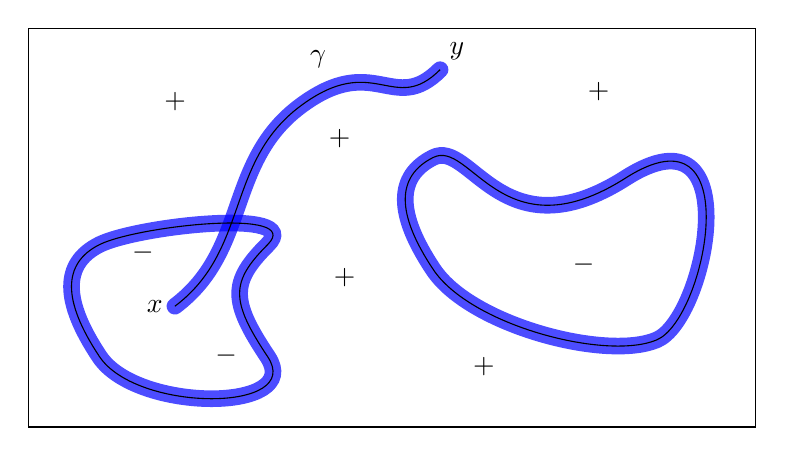
\begin{tikzpicture}[x=0.75pt,y=0.75pt,yscale=-0.9,xscale=0.9]
\draw   (10.5,78.5) -- (399.67,78.5) -- (399.67,292) -- (10.5,292) -- cycle ;
\draw [color=blue ,draw opacity=0.7 ][line width=6] (48.67,194.33) .. controls (68.67,184.33) and (158.67,174.33) .. (138.67,194.33) .. controls (118.67,214.33) and (118.67,224.33) .. (138.67,254.33) .. controls (158.67,284.33) and (68.67,284.33) .. (48.67,254.33) .. controls (28.67,224.33) and (28.67,204.33) .. (48.67,194.33) -- cycle ;
\draw   [color=blue ,draw opacity=0.7 ][line width=6, line cap = round] (89,227.33) .. controls (129,197.33) and (116,150.33) .. (156,120.33) .. controls (196,90.33) and (206,125.67) .. (231,100.67) ;
\draw  [color=blue ,draw opacity=0.7 ][line width=6] (227.33,147.67) .. controls (247.33,137.67) and (264.33,200.67) .. (330.33,158.67) .. controls (396.33,116.67) and (373.67,234) .. (347,245.33) .. controls (320.33,256.67) and (247.33,237.67) .. (227.33,207.67) .. controls (207.33,177.67) and (207.33,157.67) .. (227.33,147.67) -- cycle ;
\draw   (48.67,194.33) .. controls (68.67,184.33) and (158.67,174.33) .. (138.67,194.33) .. controls (118.67,214.33) and (118.67,224.33) .. (138.67,254.33) .. controls (158.67,284.33) and (68.67,284.33) .. (48.67,254.33) .. controls (28.67,224.33) and (28.67,204.33) .. (48.67,194.33) -- cycle ;
\draw    (89,227.33) .. controls (129,197.33) and (116,150.33) .. (156,120.33) .. controls (196,90.33) and (206,125.67) .. (231,100.67) ;
\draw   (227.33,147.67) .. controls (247.33,137.67) and (264.33,200.67) .. (330.33,158.67) .. controls (396.33,116.67) and (373.67,234) .. (347,245.33) .. controls (320.33,256.67) and (247.33,237.67) .. (227.33,207.67) .. controls (207.33,177.67) and (207.33,157.67) .. (227.33,147.67) -- cycle ;

\draw (82,111.4) node [anchor=north west][inner sep=0.75pt]    {$+$};
\draw (247.33,253.4) node [anchor=north west][inner sep=0.75pt]    {$+$};
\draw (308.67,106.07) node [anchor=north west][inner sep=0.75pt]    {$+$};
\draw (170,131.4) node [anchor=north west][inner sep=0.75pt]    {$+$};
\draw (172.67,205.4) node [anchor=north west][inner sep=0.75pt]    {$+$};
\draw (109.33,247.4) node [anchor=north west][inner sep=0.75pt]    {$-$};
\draw (64.67,192.07) node [anchor=north west][inner sep=0.75pt]    {$-$};
\draw (300.67,198.73) node [anchor=north west][inner sep=0.75pt]    {$-$};

\draw (160,89.07) node [anchor=north west][inner sep=0.75pt]    {$\gamma $};
\draw (72.67,222.73) node [anchor=north west][inner sep=0.75pt]    {$x$};
\draw (234.67,84.73) node [anchor=north west][inner sep=0.75pt]    {$y$};

\end{tikzpicture}
\caption{Open and closed defects with their loci in the spacetime. The open defect is generated by the curve $\gamma$, connecting $x$ and $y$.}
\label{fig:open-closed-defects-kink}
\end{figure}

A crucial point is to prove that $\langle s(x)s(y)\rangle$ in eq.~\eqref{eq:two-points-function-kink} depends only on $x$ and $y$ and not on $\gamma$ itself. This is a consequence of the $\Z_2$ gauge invariance, where the $\Z_2$-gauge transformations are defined as follows. Given a partition of $\R^2$ into two disjoint subsets $B$ and $B^C$ define the gauge transformation
\begin{eq}
	\big(\xi_B\phi\big)(x)=\begin{cases}
		-\phi(x)\tif x\in B\\
		+\phi(x)\tif x\in B^C
	\end{cases}
	\tand
	\xi_B\gamma=\gamma\cup\partial B
\end{eq}
where $\partial B$ is the boundary of the region $B$, moreover since $\partial B$ is necessarily closed, then $\partial(\xi_B\gamma)=\partial\gamma$. Notice that if the intersection of $\gamma$ and $\partial B$ is non-empty, then we should either consider two times the overlapping piece or neglect it in $\xi_B\gamma$ depending on whether the orientations of $\gamma$ and $\partial B$ are in the same direction or in opposite directions, similarly to what happens in the case of simplicial homology.  

Then is simple to prove that 
\begin{eq}
	\nabla^{\xi_B\gamma}(\xi_B\phi)=\xi_B(\nabla^\gamma\phi)
\end{eq}
and
\begin{eq}
	(\xi_B\phi)^{2n}=\phi^{2n}
\end{eq}
therefore
\begin{eq}
	S^{\xi_B\gamma}(\xi_B\phi)=S^\gamma(\phi)
\end{eq}
Furthermore, we clearly have
\begin{eq}
	\pide\phi=\pide(\xi_B\phi)
\end{eq}
provided that $B$ is compact.

Since we can deform arbitrarily \todo{Ma se due defect possono interagire solo se vicini, cosa succede se prendiamo due $\gamma_i$ vicini e li deformiamo fino ad averli arbitrariamente lontani? In un caso dovrebbero interagire mentre nell'altro no, ma ciò non è consistente con la nostra simmetria, quindi l'unica soluzione sarebbe che i defect non possano interagire...} $\gamma$ acting on it with several $\Z_2$-transformations with different choices of $B$, provided that $x$ and $y$ are fixed (indeed $\partial(\xi_B\gamma)=\partial\gamma$ implies that $x$ and $y$ cannot change under $\xi_B$), then the invariance of $S^\gamma$ and $\pide\phi$ under $\xi_B$ implies that eq.~\eqref{eq:two-points-function-kink} depends only on $x$ and $y$ and not on $\gamma$, as desired. 

\subsubsection{The reconstruction of the kink operator}

One can prove that a natural generalization of the above construction of the correlator for an arbitrary even number of points (correlators of an odd number of points are set to zero) satisfy the OS axioms, hence we can reconstruct a quantum kink field operator $\op s(x)$ which create and destroy kinks, such that
\begin{eq}
	\bra\Omega\op s(\vec x)e^{-(x^0-y^0)H}\op s(\vec y)\ket\Omega=\langle s(x) s(y)\rangle
\end{eq}

One can prove (rigorously in the lattice approximation) that $\op s(x)$ couple to the vacuum $\ket\Omega$ to a one-particle state, so that $\op s(x)$ really creates and annihilate kink particles, which for this reason should be included in scattering states. 


\subsubsection{The insertion of the meson field - The dual algebra}

Notice that up to now we only considered the QFT description of the soliton, but in our theory we can also describe the creation and the annihilation of particles associated to the original scalar field, not in the broken symmetry phase, describing the mesons. The QFT description of such particles is just the usual $\phi_4$ theory, and we can describe the associated operators without any difficulty computing the correlation functions in the Euclidean spacetime satisfying OS axioms. However describing a theory involving both kinks and mesons is more involved. 

First of all, notice that the field $\phi(x)$ is not $\Z_2$-gauge invariant, however we can define a new field
\begin{eq}
	\phi_\gamma(x):=\phi(x)\,U(\omega_x\vert\gamma)
\end{eq}
 where $\omega_x$ is a straight line at constant Euclidean time from $x$ to $+\infty$, as shown in fig.~\ref{fig:omega_x}, which is $\Z_2$-gauge invariant. 

\begin{figure}[h]
\centering
\tikzstyle{arrow} = [thick,->,>=stealth]
\begin{tikzpicture}[xscale=0.5,yscale=0.5]
\draw [arrow] (0,0.5) -- (0,4.5);
\draw (2,2) -- (8,2);
\draw (8.2,2) -- (8.4,2);
\draw (8.6,2) -- (8.8,2);
\draw (-0.1,2) -- (0.1,2);
\draw (2,2) circle (2pt)[fill=black] ;
\draw (2,2.6) node {$x$};
\draw (9.8,2) node {$+\infty$};
\draw (7,1.5) node {$\omega_x$};
\draw (-0.5,4.3) node {$\tau$};
\draw (-0.5,2) node {$x^0$};
\end{tikzpicture}
\caption{Representation of the line $\omega_x$.}
\label{fig:omega_x}
\end{figure}

With the insertion of $\phi_\gamma(x)$ the correlation functions become
\begin{eq}
	\langle s(x)s(y)\phi(z)\phi(w)\rangle=\frac{\int\pide\phi\,e^{-S_\gamma(\phi)}\phi_\gamma(z)\phi_\gamma(w)}{\int\pide\phi\,e^{-S_\gamma(\phi)}}
\end{eq}
with $\gamma$ line from $x$ to $y$, and satisfy OS axioms except for the symmetry property between kink and meson insertions, which means that the quantum field $\ophi( x)$ and $\op s(z)$ are not relatively local. 

However it is easy to see that if we consider the insertion of the kink at $x^{\pm\epsilon}=(x^0=\pm\epsilon,x^1)$ and the insertion of the meson at $y=(y^0=0,y^1)$ and we denote by\footnote{The first $2n$ variables denotes the boundaries of $n$ curves $\gamma_1,\ldots,\gamma_n$, describing the solitons, and the last $m$ variables denotes the insertion points of the $m$ mesons.} $S^{2n,m}(x_1,\ldots,x_{2n};y_1,\ldots,y_m)$ the Schwinger functions for $2n$ kinks and $m$ mesons we get
\begin{eq}\label{eq:schwinger-dual-algebra-kink}
	\lim_{\epsilon\to0}S^{2n,m}(\ldots,x^\epsilon;y,\ldots)=\lim_{\epsilon\to0}(-1)^{\theta(x^1-y^1)}S^{2n,m}(\ldots,x^{-\epsilon};y,\ldots)
\end{eq}
so that the reconstructed fields satisfy a new commutation relation called \emph{dual algebra}\footnote{Such new algebra appeared for the first time in \cite{Frohlich1976}.}
\begin{eq}\label{eq:dual-algebra}
	\op s(x^1)\ophi(y^1)=(-1)^{\theta(x^1-y^1)}\ophi(y^1)\op s(x^1)
\end{eq}
where $\theta$ is the Heaviside step function, proving that among fields of a relativistic QFT are possible also such ``strange'' commutation relations in presence of solitons. 

Let us motivate eq.~\eqref{eq:schwinger-dual-algebra-kink} at least graphically. We start from the case $x^1>y^1$. If we insert a kink in $x^\epsilon$ and a meson at $y$, the situation is the following 

\vspace{-0.5cm}
\begin{figure}[H]
\centering
\tikzstyle{arrow} = [thick,->,>=stealth]
\begin{tikzpicture}[xscale=0.5,yscale=0.5]
\clip (-1,0) rectangle + (12.5,5);
\draw [arrow] (0,0) -- (0,4.5);
\draw (2,2) -- (8,2);
\draw (8.2,2) -- (8.4,2);
\draw (8.6,2) -- (8.8,2);
\draw (-0.1,2) -- (0.1,2);
\draw (-0.1,2.7) -- (0.1,2.7);
\draw (2,2) circle (2pt)[fill=black] ;
\draw (4,2.7) circle (2pt)[fill=black] ;
\draw (2,2.6) node {$y$};
\draw (9.8,2) node {$+\infty$};
\draw (7,1.5) node {$\omega_{y}$};
\draw (-0.5,4.3) node {$\tau$};
\draw (-0.5,2) node {$0$};
\draw (-0.5,2.7) node {$\epsilon$};
\draw (4.5,3.3) node {$x^{\epsilon}$};
\end{tikzpicture}
\end{figure}
\vspace{-0.3cm}

whereas, inserting the kink in $x^{-\epsilon}$ we get

\begin{figure}[H]
\centering
\tikzstyle{arrow} = [thick,->,>=stealth]
\begin{tikzpicture}[xscale=0.5,yscale=0.5]
\clip (-1,0) rectangle + (12.5,5);
\draw [arrow] (0,0) -- (0,4.5);
\draw (2,2) -- (8,2);
\draw (8.2,2) -- (8.4,2);
\draw (8.6,2) -- (8.8,2);
\draw (-0.1,2) -- (0.1,2);
\draw (-0.1,1.3) -- (0.1,1.3);
\draw (2,2) circle (2pt)[fill=black] ;
\draw (4,1.3) circle (2pt)[fill=black] ;
\draw (2,2.6) node {$y$};
\draw (9.8,2) node {$+\infty$};
\draw (7,1.5) node {$\omega_{y}$};
\draw (-0.5,4.3) node {$\tau$};
\draw (-0.5,2) node {$0$};
\draw (-0.7,1.3) node {$-\epsilon$};
\draw (5,1.5) node {$x^{-\epsilon}$};
\end{tikzpicture}
\end{figure}

Now we have to fix the second boundary point defining the open defect of the kink, and suppose without loss of generality that such point has time coordinate strictly smaller than $-\epsilon$. Then the we get

\begin{figure}[H]
\centering
\tikzstyle{arrow} = [thick,->,>=stealth]
\begin{tikzpicture}[xscale=0.5,yscale=0.5]
\clip (-1,0) rectangle + (12.5,5);
\draw [arrow] (0,0) -- (0,4.5);
\draw (2,2) -- (8,2);
\draw (8.2,2) -- (8.4,2);
\draw (8.6,2) -- (8.8,2);
\draw (-0.1,2) -- (0.1,2);
\draw (-0.1,2.7) -- (0.1,2.7);
\draw (4,2.7) -- (4,0.8);
\draw (4,0.6) -- (4,0.4);
\draw (4,0.2) -- (4,0);
\draw (2,2) circle (2pt)[fill=black] ;
\draw (4,2.7) circle (2pt)[fill=black] ;
\draw (2,2.6) node {$y$};
\draw (9.8,2) node {$+\infty$};
\draw (7,1.5) node {$\omega_{y}$};
\draw (-0.5,4.3) node {$\tau$};
\draw (-0.5,2) node {$0$};
\draw (-0.5,2.7) node {$\epsilon$};
\draw (4.5,3.3) node {$x^{\epsilon}$};
\draw (3.5,1) node {$\gamma$};
\end{tikzpicture}
\end{figure}

and

\begin{figure}[H]
\centering
\tikzstyle{arrow} = [thick,->,>=stealth]
\begin{tikzpicture}[xscale=0.5,yscale=0.5]
\clip (-1,0) rectangle + (12.5,5);
\draw [arrow] (0,0) -- (0,4.5);
\draw (2,2) -- (8,2);
\draw (8.2,2) -- (8.4,2);
\draw (8.6,2) -- (8.8,2);
\draw (-0.1,2) -- (0.1,2);
\draw (-0.1,1.3) -- (0.1,1.3);
\draw (4,1.3) -- (4,0.8);
\draw (4,0.6) -- (4,0.4);
\draw (4,0.2) -- (4,0);
\draw (2,2) circle (2pt)[fill=black] ;
\draw (4,1.3) circle (2pt)[fill=black] ;
\draw (2,2.6) node {$y$};
\draw (9.8,2) node {$+\infty$};
\draw (7,1.5) node {$\omega_{y}$};
\draw (-0.5,4.3) node {$\tau$};
\draw (-0.5,2) node {$0$};
\draw (-0.7,1.3) node {$-\epsilon$};
\draw (5,1.5) node {$x^{-\epsilon}$};
\draw (3.5,0.8) node {$\gamma$};
\end{tikzpicture}
\end{figure}

so that in the first case $U(\omega_y\vert\gamma)=-1$ whereas in the second one $U(\omega_y\vert\gamma)=1$. Taking the limit $\epsilon\to0$ this implies (see the references) eq.~\eqref{eq:schwinger-dual-algebra-kink} in the case $x^1>y^1$. Instead, in the case $x^1<y^1$, the situation in the following: 

\begin{figure}[H]
\centering
\tikzstyle{arrow} = [thick,->,>=stealth]
\begin{tikzpicture}[xscale=0.5,yscale=0.5]
\clip (-1,0) rectangle + (12.5,5);
\draw [arrow] (0,0) -- (0,4.5);
\draw (4,2) -- (8,2);
\draw (8.2,2) -- (8.4,2);
\draw (8.6,2) -- (8.8,2);
\draw (-0.1,2) -- (0.1,2);
\draw (-0.1,2.7) -- (0.1,2.7);
\draw (2,2.7) -- (2,0.8);
\draw (2,0.6) -- (2,0.4);
\draw (2,0.2) -- (2,0);
\draw (4,2) circle (2pt)[fill=black] ;
\draw (2,2.7) circle (2pt)[fill=black] ;
\draw (4,2.6) node {$y$};
\draw (9.8,2) node {$+\infty$};
\draw (7,1.5) node {$\omega_{y}$};
\draw (-0.5,4.3) node {$\tau$};
\draw (-0.5,2) node {$0$};
\draw (-0.5,2.7) node {$\epsilon$};
\draw (2.5,3.3) node {$x^{\epsilon}$};
\draw (1.5,1) node {$\gamma$};
\end{tikzpicture}
\end{figure}

and

\begin{figure}[H]
\centering
\tikzstyle{arrow} = [thick,->,>=stealth]
\begin{tikzpicture}[xscale=0.5,yscale=0.5]
\clip (-1,0) rectangle + (12.5,5);
\draw [arrow] (0,0) -- (0,4.5);
\draw (4,2) -- (8,2);
\draw (8.2,2) -- (8.4,2);
\draw (8.6,2) -- (8.8,2);
\draw (-0.1,2) -- (0.1,2);
\draw (-0.1,1.3) -- (0.1,1.3);
\draw (2,1.3) -- (2,0.8);
\draw (2,0.6) -- (2,0.4);
\draw (2,0.2) -- (2,0);
\draw (4,2) circle (2pt)[fill=black] ;
\draw (2,1.3) circle (2pt)[fill=black] ;
\draw (4,2.6) node {$y$};
\draw (9.8,2) node {$+\infty$};
\draw (7,1.5) node {$\omega_{y}$};
\draw (-0.5,4.3) node {$\tau$};
\draw (-0.5,2) node {$0$};
\draw (-0.7,1.3) node {$-\epsilon$};
\draw (3,1.5) node {$x^{-\epsilon}$};
\draw (1.5,0.8) node {$\gamma$};
\end{tikzpicture}
\end{figure}

In this case $U(\omega_y\vert\gamma)=U(\omega_y\vert\gamma)=1$, and we get eq.~\eqref{eq:schwinger-dual-algebra-kink} in the case $x^1<y^1$.

\skipline

Notice that eq.~\eqref{eq:dual-algebra} give a new type of commutation relations, different respect both bosonic and fermionic ones, which depend on the space coordinates. Such statistics is very similar to the \emph{braid statistic}, which differs from this case since in the case of braid statistic the phase introduced in the commutation relation depends on whether the particles are interchanged in the clockwise or in the anticlockwise direction. 
It worth to highlight the fact that the existence of both these statistics depends on the possibility of give a well-define ordering of the points of our spacetime. For instance in $D=3+1$ such statistics cannot exists, at least for massive particles. 
The factor $(-1)^{\theta(x^1-y^1)}$ in eq.~\eqref{eq:dual-algebra} provides the $R$-matrix representation of the braid group. 

%%%%%%%%%%%%%%%%%%%%%%%
%%%%%%%% LECTURE 16 PART 1%%%%%%%%
%%%%%%%%%%%%%%%%%%%%%%%

\subsubsection{The fermionic excitations}

Let us define a new field
\begin{eq}
	\opsi(x):=\ophi(x)\op s(x)
\end{eq}
then we have (writing $x^1$ instead of $(0,x^1)$, same for $y_1$)
\begin{eq}
	\opsi(x^1)\opsi(y^1)
	&=\ophi(x^1)\op s(x^1)\ophi(y^1)\op s(y^1)\\
	&=(-1)^{\theta(x^1-y^1)}\ophi(x^1)\ophi(y^1)\op s(x^1)\op s(y^1)\\
	&=(-1)^{\theta(x^1-y^1)}\ophi(y^1)\ophi(x^1)\op s(y^1)\op s(x^1)\\
	&=(-1)^{\theta(x^1-y^1)}(-1)^{\theta(y^1-x^1)}\ophi(y^1)\op s(y^1)\ophi(x^1)\op s(x^1)\\
	&=-\opsi(x^1)\opsi(y^1)
\end{eq}
hence $\opsi$ describes a fermionic field, hence the theory admits fermionic excitations. 

The operator $\opsi$ is the analogue of the Onsager fermion field at the critical point in the Ising model, with the difference that the Onsager field is free whereas $\opsi$ describes a strongly interacting field. 

\subsubsection{The reconstructed Hilbert space}

We now discuss which is the relation between the kink operator and the classical kink solution. Let us compute the expectation value of $\ophi(y^1)$ in presence of the kink operator, in particular we compute\footnote{The factor $e^{-\epsilon H}$ comes from the proof the the OS reconstruction theorem.}
\begin{eq}\label{eq:exp-value-QFT-kink}
	\tilde\phi_S(x^1,y^1)
	\frac { \bra{e^{-\epsilon H}\op s(x^1)\Omega}\ophi(y^1)\ket{e^{-\epsilon H}\op s(x^1)\Omega} }
	        { \braket{e^{-\epsilon H}\op s(x^1)\Omega}{e^{-\epsilon H}\op s(x^1)\Omega} }
\end{eq}
The numerator in the previous expression can be represented by 
%
\begin{figure}[H]
\centering
\tikzstyle{arrow} = [thick,->,>=stealth]
\begin{tikzpicture}[xscale=0.5,yscale=0.5]
\clip (-1,0) rectangle + (12.5,5);
\draw [arrow] (0,0) -- (0,4.5);
\draw (2,2) -- (8,2);
\draw (8.2,2) -- (8.4,2);
\draw (8.6,2) -- (8.8,2);
\draw (-0.1,2) -- (0.1,2);
\draw (-0.1,3.1) -- (0.1,3.1);
\draw (-0.1,0.9) -- (0.1,0.9);
\draw (4,3.1) -- (4,0.9);
\draw (2,2) circle (2pt)[fill=black] ;
\draw (4,3.1) circle (2pt)[fill=black] ;
\draw (4,0.9) circle (2pt)[fill=black] ;
\draw (2,2.6) node {$y$};
\draw (9.8,2) node {$+\infty$};
\draw (7,1.5) node {$\omega_{y}$};
\draw (-0.5,4.3) node {$\tau$};
\draw (-0.5,2) node {$0$};
\draw (-0.5,3.1) node {$\epsilon$};
\draw (-0.7,0.9) node {$-\epsilon$};
\draw (4.5,3.7) node {$x^{\epsilon}$};
\draw (5,1.1) node {$x^{-\epsilon}$};
\draw (3.6,1.4) node {$\gamma$};
\end{tikzpicture}
\end{figure}
%
so that $\tilde \phi_S$ must have a zero at $x^1$, since at the defect $\gamma$ the field changes sign. 
If we impose positive boundaries conditions for the field: $\bra\Omega\ophi\ket\Omega=\phi_+$, then
\begin{eq}
	\phi_\gamma(y^1)=\phi(y^1)U(\omega_y,\gamma)\to\pm\phi(y^1)
	\tfor
	y^1\to\pm\infty
\end{eq}
since $\omega_y$ either does not intersect $\gamma$ or intersect it certainly. Then by cluster property we have 
\begin{eq}
	\bra{e^{-\epsilon H}\op s(x^1)\Omega}\ophi(y^1\to\pm\infty)\ket{e^{-\epsilon H}\op s(x^1)\Omega} 
	\quad\to\quad
	\phi_\pm \braket{e^{-\epsilon H}\op s(x^1)\Omega}{e^{-\epsilon H}\op s(x^1)\Omega}
\end{eq}
so that $\phi_S(x,y)$ defined in eq.~\eqref{eq:exp-value-QFT-kink} behaves topologically (that is, at boundaries) as the classical kink with coordinate $y^1$ and modulus $x^1$, which we denoted by $\phi_S(y^1-x^1)$:
\begin{eq}
	\tilde \phi_S(x,y) \simeq \phi_S(y^1-x^1)
\end{eq}

\skipline

With positive boundaries conditions the reconstruction theorem proves that the Hilbert space can be separated in a vacuum sector  and a kink sector
\begin{eq}
	\hs=\hs_+\oplus\hs_S
	\twith
	\ket\Omega\in\hs_+
	\tand
	\op s(x)\ket\Omega\in\hs_S
\end{eq}
The direct sum (hence the non-interference between elements of the two spaces) is due to the fact that there are no inner products between an even and an odd number of solitons states, because the correlation function with an odd number of kink insertion vanish,\footnote{This may be motivated as follows: we know that a kink is described by a open line defect, hence is associated to two points. The only configuration of the defects which allows for an odd number of insertion points is the one where one (or more) open defect $\gamma$ connects a point $z$ in the spacetime to the boundary $\infty$. However, since the kink carries a mass, the energy required to move the kink from $z$ to $\infty$ is proportional to $m_{\text{kink}}\cdot\text{length}(\gamma)=\infty$. This of course holds in the broken symmetry phase, as otherwise any transformation (including translations to arbitrary points of the spacetime) are physically allowed.} and clearly $\op s$ maps vectors of $\hs_+$ in vectors of $\hs_S$, $\op s(x):\hs_+\to\hs_S$. This can be equivalently stated saying that $\hs_S$ is a \emph{superselection sector}. 

\skipline

\todo{Temo che in questo paragrafo non sia ben chiaro il concetto, penso che qualche chiarimento sia utile.}
In the ``unbroken'' original $\Z_2$-phase, it turns out that $\hs$ cannot be separated in the direct sum of two subspaces. Let us show why. If the $\Z_2$ symmetry is restored, then all possible configurations are closed to the vacuum $\phi_0$, and since all transformations are physically allowed it is much easier to find configurations where $\phi$ vanishes. Hence there are much more defects respect to the broken-phase case, and typically the net of defects (the collection of regions where $\phi$ vanishes) reaches the boundary $\infty$ of the spacetime. If this is the case, then an additional line defect $\gamma$ from $z$ to $\infty$ cannot affect the correlation function. 

But then by the cluster property the kink position sent to infinity is incompatible with $\bra{\Omega}\op s(x\to\infty)\ket{\Omega}=0$. Hence the Hilbert space $\hs$ has no superselection kink sectors, $\hs\equiv\hs_0$, and the phase in which the net of defects reaches the infinity corresponds to the unbroken $\Z_2$-symmetry.  

The configuration, which appears in the unbroken phase, in which the defects almost covers the whole space time, is said \emph{condensation of kinks}. 

\skipline

By reconstruction theorem we know that in $\hs$ there is a unitary representation of the Poincaré group, which in turn implies that we have unitary representation of the Poincaré group also in both $\hs_+$ and $\hs_S$.  Recall that at classical level the modulus of the kink breaks translational invariance, which at the level of quantum mechanics is recovered by promoting the modulus to a quantum coordinate. In the QFT framework, instead, translational invariance is recovered directly in the proof of the OS reconstruction theorem.
By uniqueness of the vacuum, there are no translational invariant vector states in $\hs_S$ (as the only one is the vacuum, which is an element of $\hs_+$). 

\end{document}